\section{Exercises}

%%%%%%%%%%%%%%%%%%%%%

\subsection{Line fitting, residuals, and correlation}

%%%%%%%%%%%%%%%%%%%%%

% 1

\eoce{The scatterplots shown below each have a superimposed regression line. If we were to construct a residual plot (residuals versus $x$) for each, what would those plots look like?
\begin{center}
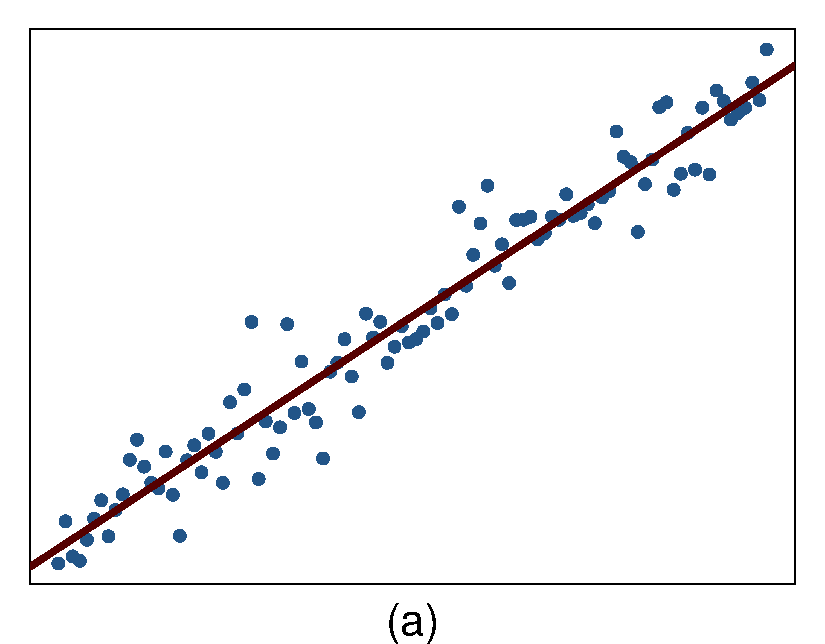
\includegraphics[width=0.49\textwidth]{07/figures/eoce/resDemoLin.pdf} 
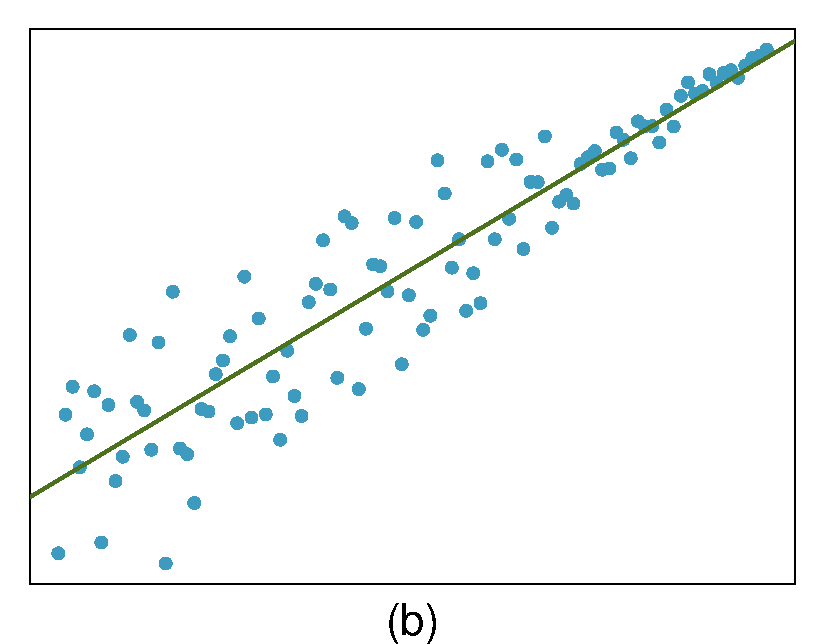
\includegraphics[width=0.49\textwidth]{07/figures/eoce/resDemoFanBack.pdf}
\end{center}
}
{
\begin{enumerate}[(a)]
\item The relationship is linear therefore the residuals plot will show randomly distributed residuals around 0 with constant variance.
\item The scatterplot shows a fan shape, with higher variability in $y$ for lower $x$. Therefore the residuals plot will also show a fan shape, wider around lower $x$, narrower around higher $x$. There may also be characteristics indicating nonlinearity for points on the left.
\end{enumerate}
Note: Below are the residuals plots.
\begin{center}
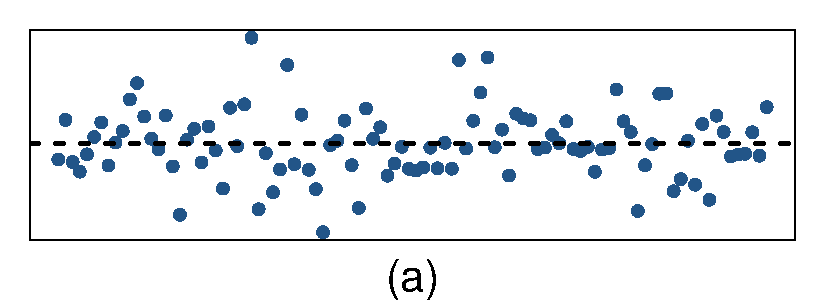
\includegraphics[width=0.49\textwidth]{07/figures/eoce/resDemoResScatLin.pdf}
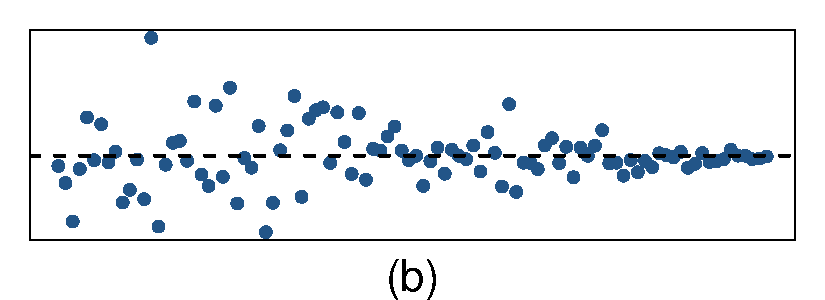
\includegraphics[width=0.49\textwidth]{07/figures/eoce/resDemoResScatFanBack.pdf} \\
\end{center}
}

% 2

\eoce{Shown below are two plots of residuals remaining after fitting a linear model to two different sets of data. Describe any apparent trends in these plots and determine if a linear model would be appropriate for these data. Explain your reasoning.
\begin{center}
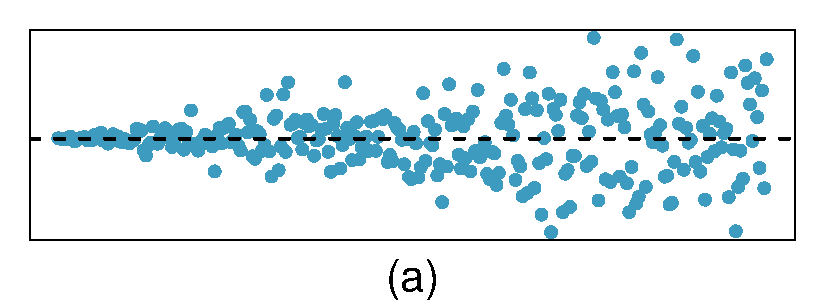
\includegraphics[width=0.49\textwidth]{07/figures/eoce/resDemoResScatFan.pdf} 
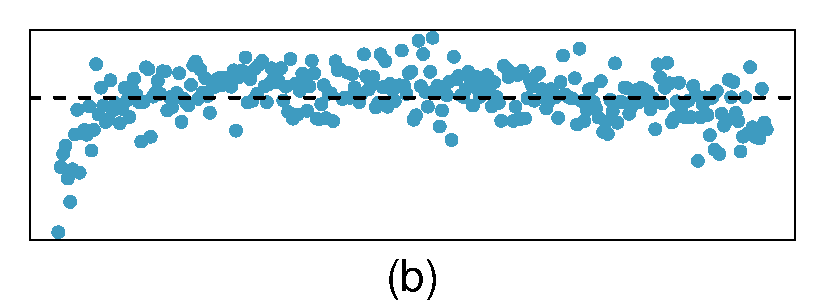
\includegraphics[width=0.49\textwidth]{07/figures/eoce/resDemoResScatExp.pdf}
\end{center}
}
{
\begin{enumerate}[(a)]
\item There is a fan shape in the residuals plot, therefore we would expect a fan shape in the scatterplot  of $y$ versus $x$ as well. Variability around the regression line will increase as $x$ increases. Since there is a trend in the residuals plot a linear model would using the methods we have described not be appropriate for these data.
\item There is an apparent curvature in the residuals plot meaning that the relationship between $x$ and $y$ variables is also curved. Therefore a linear model would not be appropriate for these data.
\end{enumerate}
%Note: Below are scatterplots of the data sets.
%\begin{center}
%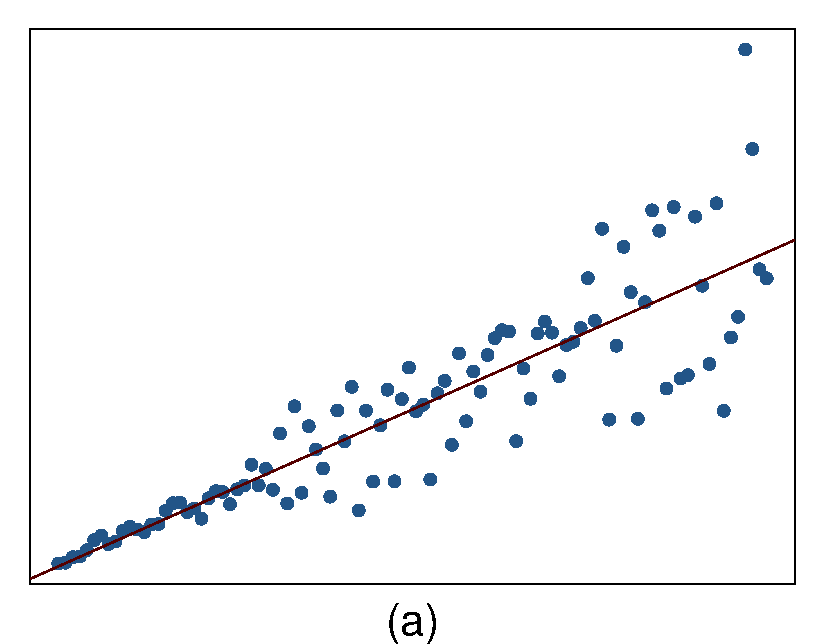
\includegraphics[width=0.49\textwidth]{07/figures/eoce/resDemoFan.pdf}
%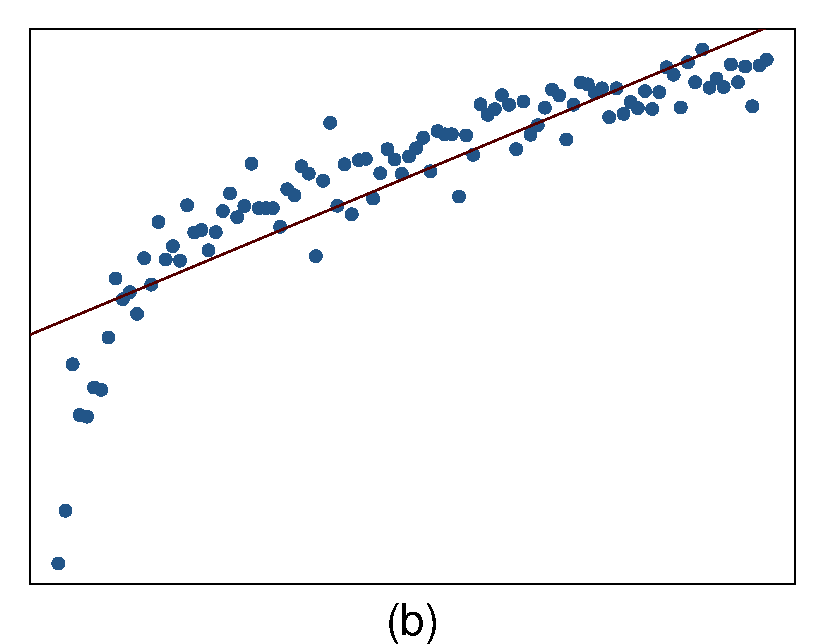
\includegraphics[width=0.49\textwidth]{07/figures/eoce/resDemoExp.pdf} 
%\end{center}
}

% 3

\eoce{For each of the six plots, identify the strength of the relationship (e.g. weak, moderate, or strong) in the data and whether fitting a linear model would be reasonable.
\begin{center}
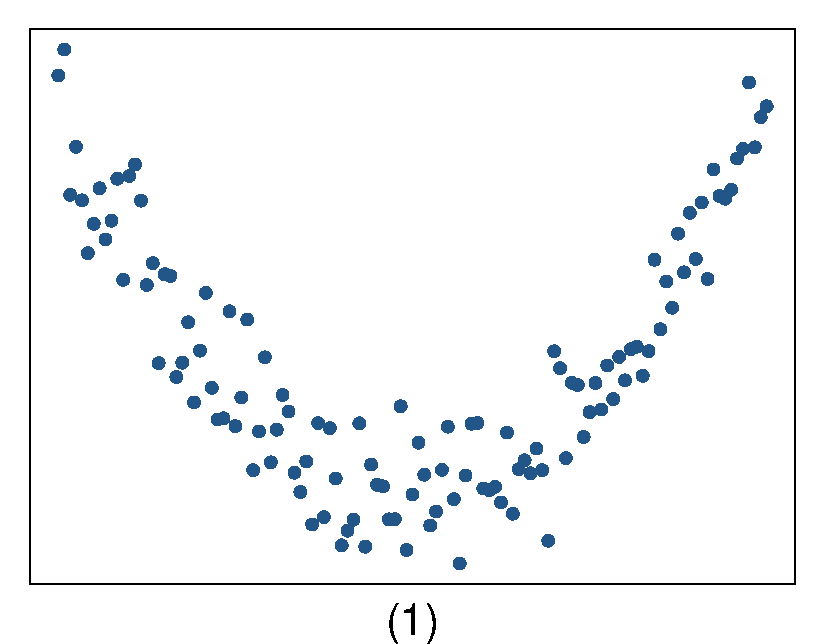
\includegraphics[width=0.32\textwidth]{07/figures/eoce/association1.pdf}
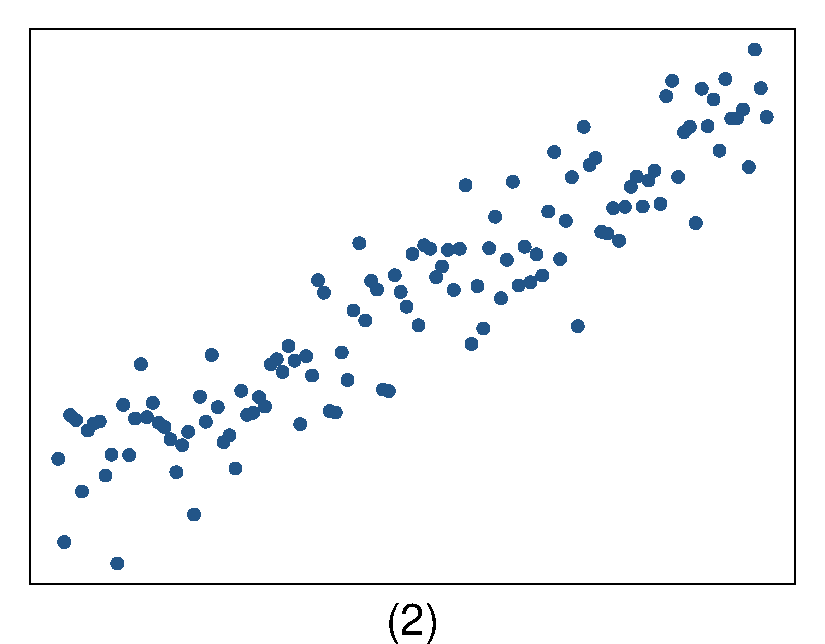
\includegraphics[width=0.32\textwidth]{07/figures/eoce/association2.pdf}
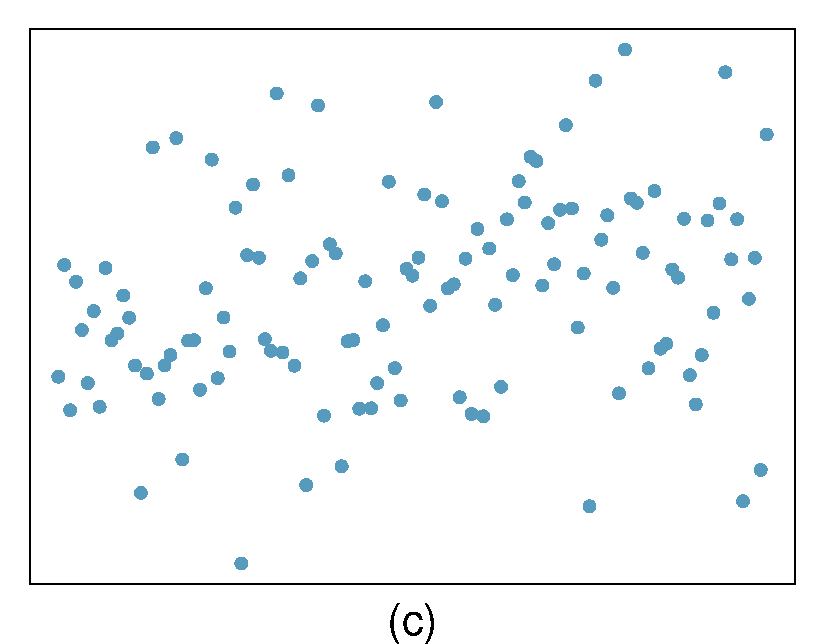
\includegraphics[width=0.32\textwidth]{07/figures/eoce/association3.pdf}
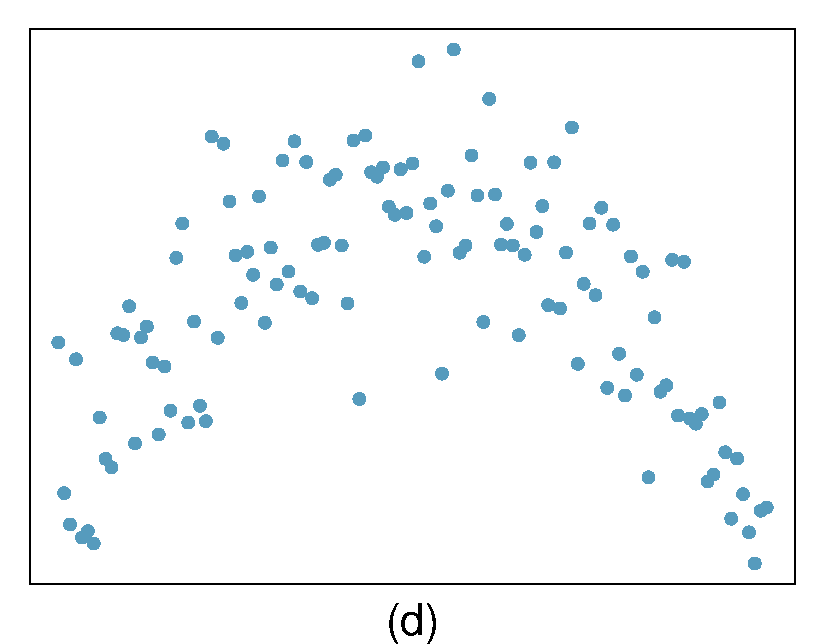
\includegraphics[width=0.32\textwidth]{07/figures/eoce/association4.pdf}
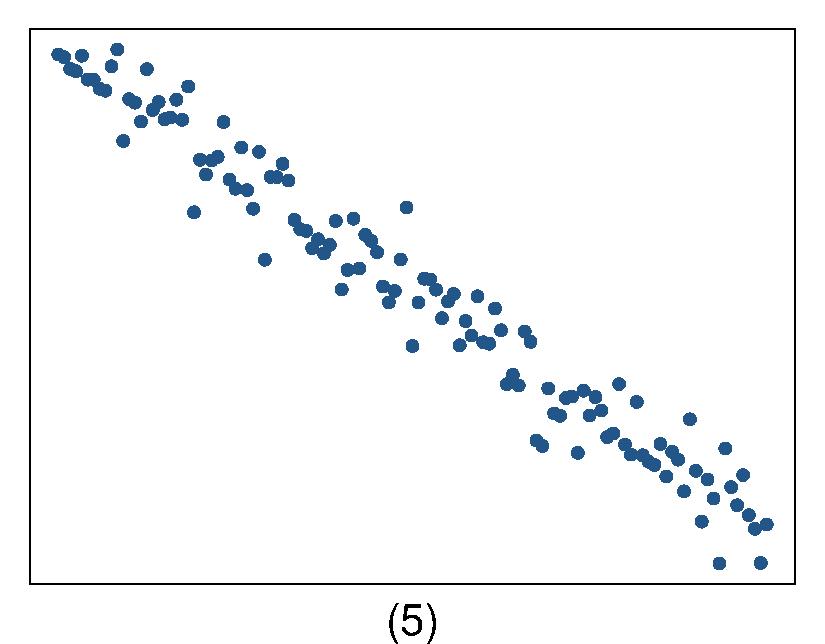
\includegraphics[width=0.32\textwidth]{07/figures/eoce/association5.pdf}
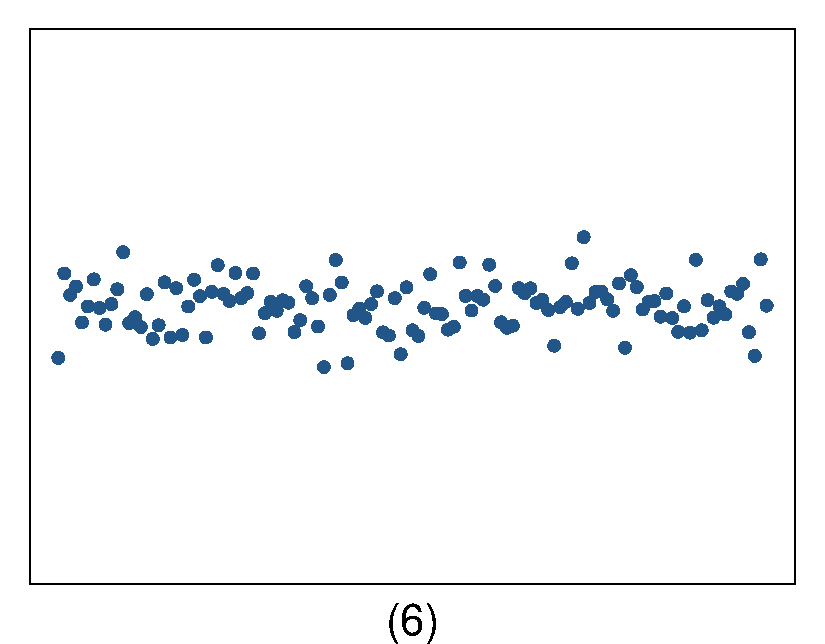
\includegraphics[width=0.32\textwidth]{07/figures/eoce/association6.pdf}
\end{center}
}
{
(2) and (5) show a strong correlation. Even though (1) and (4) show a strong association, the relationship is not linear therefore correlation would not be strong. (3) and (6) show very weak or no relationship. Answers may vary slightly, e.g. one person�s \emph{moderate} may be equivalent to another person�s \emph{strong}.
}

% 4

\eoce{For each of the six plots, identify the strength of the relationship (e.g. weak, moderate, or strong) in the data and whether fitting a linear model would be reasonable.
\begin{center}
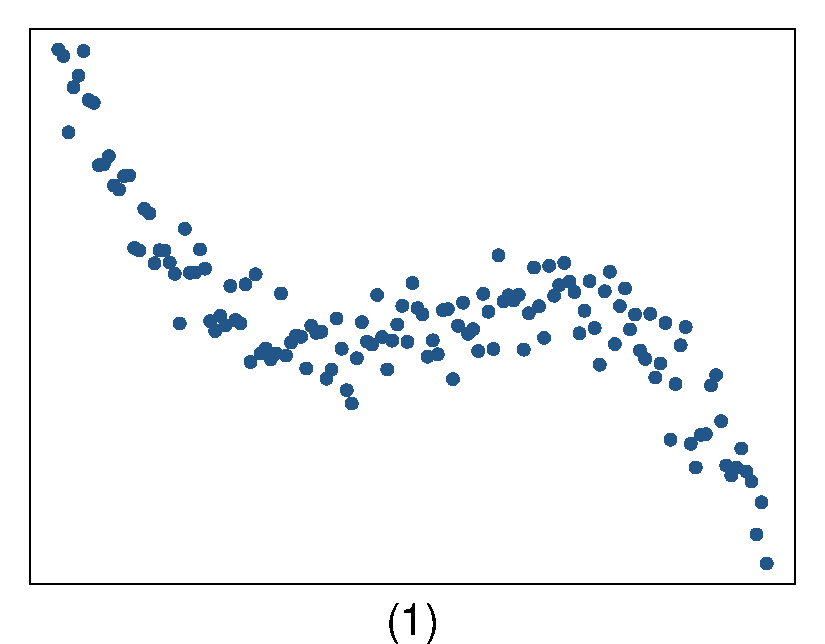
\includegraphics[width=0.32\textwidth]{07/figures/eoce/association7.pdf}
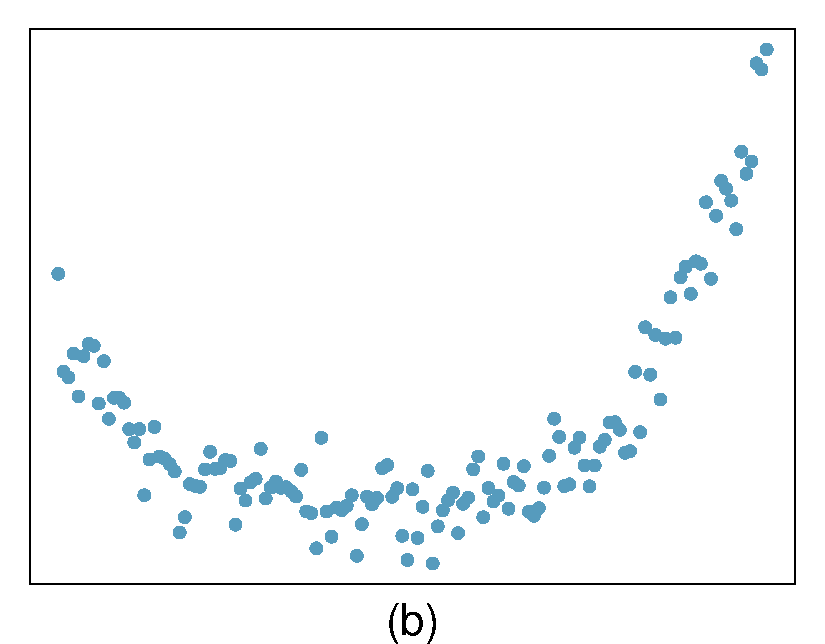
\includegraphics[width=0.32\textwidth]{07/figures/eoce/association8.pdf}
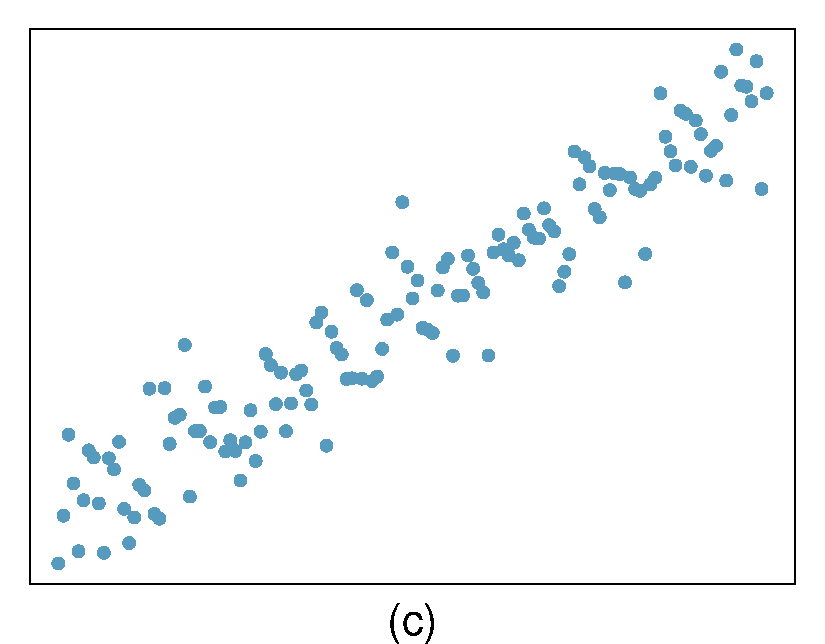
\includegraphics[width=0.32\textwidth]{07/figures/eoce/association9.pdf}
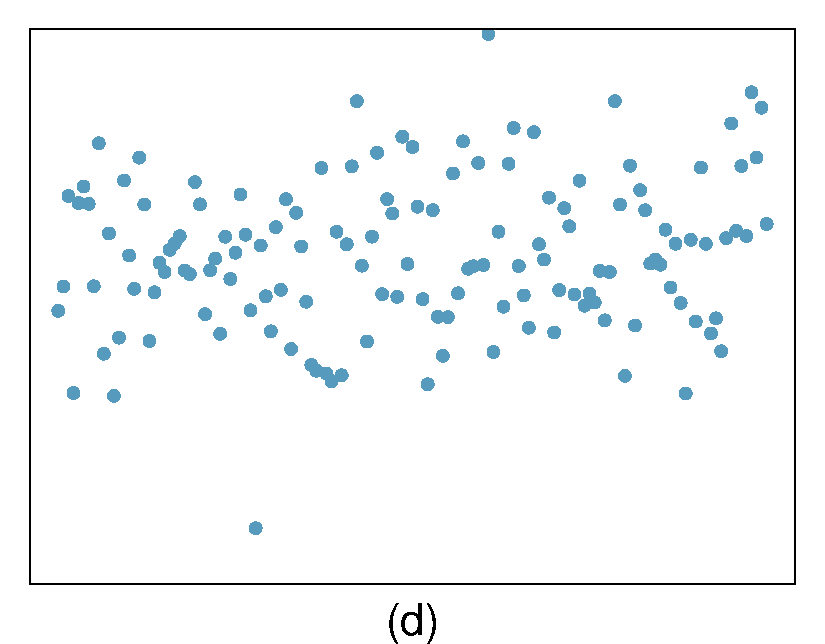
\includegraphics[width=0.32\textwidth]{07/figures/eoce/association10.pdf}
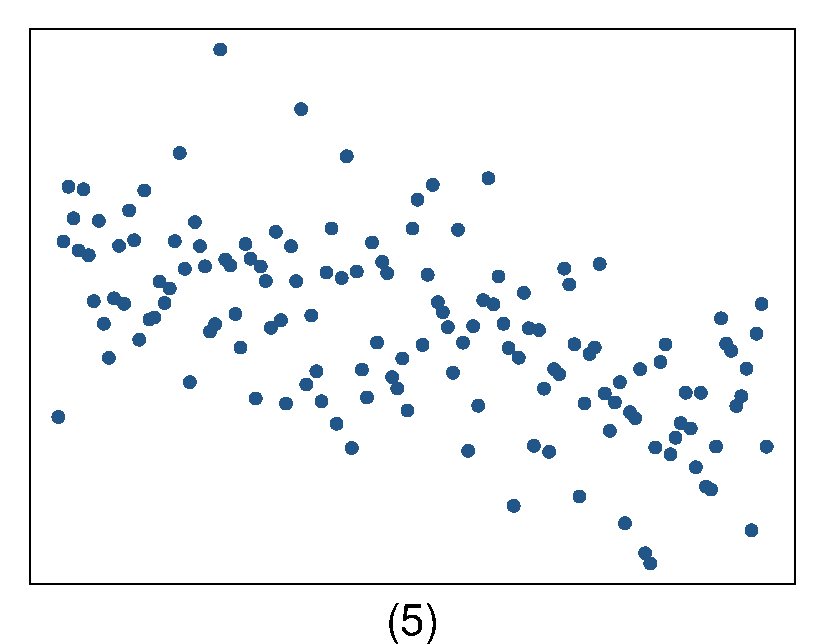
\includegraphics[width=0.32\textwidth]{07/figures/eoce/association11.pdf}
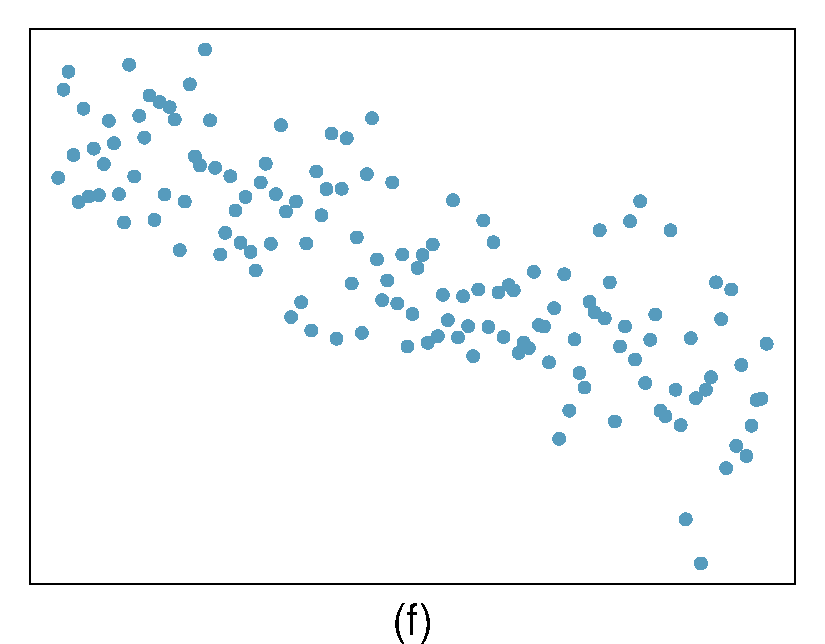
\includegraphics[width=0.32\textwidth]{07/figures/eoce/association12.pdf}
\end{center}
}
{
(3) and (6) show a strong correlation. Even though (1) and (2) show a strong association, the relationship is not linear therefore correlation would not be strong. (4) and (5) show very weak relationship. Answers may vary slightly, e.g. one person�s \emph{moderate} may be equivalent to another person�s \emph{strong}.
}

% 5

\eoce{Below are two scatterplots based on grades recorded during several years for a Statistics course at a university. The first plot shows a scatterplot for final exam grade versus first exam grade for 233 students, and the second scatterplot shows the final exam grade versus second exam grade. 
\begin{enumerate}[(a)]
\setlength{\itemsep}{0mm}
\item Based on these graphs, which of the two exams has the strongest correlation with the final exam grade? Explain.
\item Can you think of a reason why the correlation between the exam you chose in part (a) and the final exam is higher?
\end{enumerate}
\begin{center}
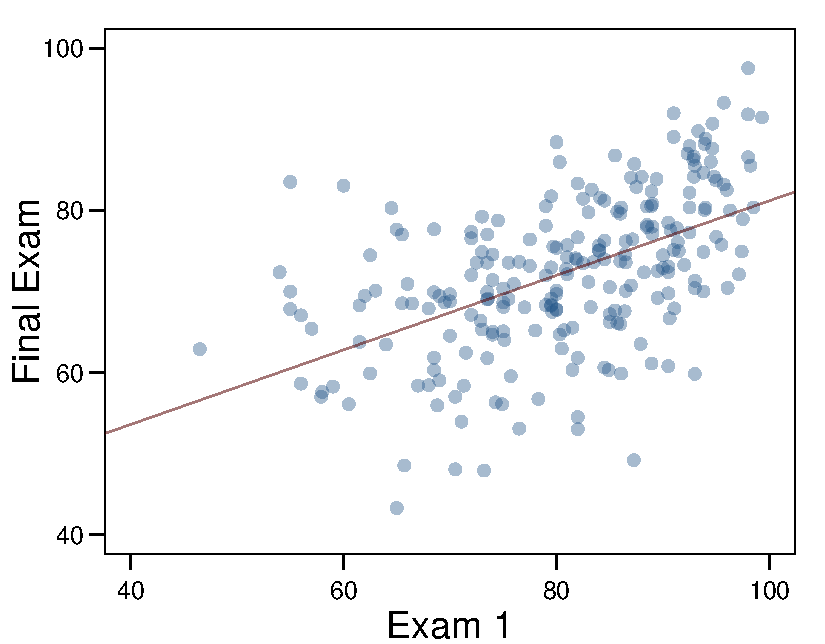
\includegraphics[width=0.49\textwidth]{07/figures/eoce/examGrades1.pdf}\ \ 
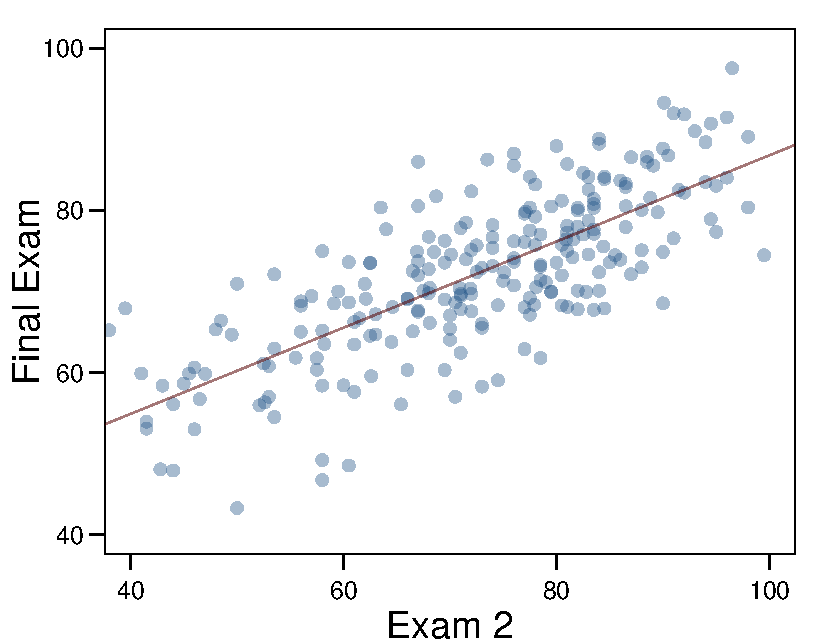
\includegraphics[width=0.49\textwidth]{07/figures/eoce/examGrades2.pdf}
\end{center}
}
{
\begin{enumerate}[(a)]
\item Exam 2 since there is less of a scatter in the plot of final exam grade versus exam 2. The correlation coefficient between these two variables would be higher than the correlation between exam 1 and course grade.
\item Exam 2 and the final are relatively close to each other chronologically, or Exam 2 may be cumulative so has greater similarities in material to the final exam.
\end{enumerate}
}

\pagebreak
% 6

\eoce{The Great Britain Office of Population Census and Surveys once collected data on a random sample of 170 married couples in Britain, recording the age (in years) and heights (converted here to inches) of the husbands and wives \citep{Hand:1994}. The scatterplot on the left shows the wife's age plotted against her husband's age, and the plot on the right shows wife's height plotted against husband's height. 
\begin{center}
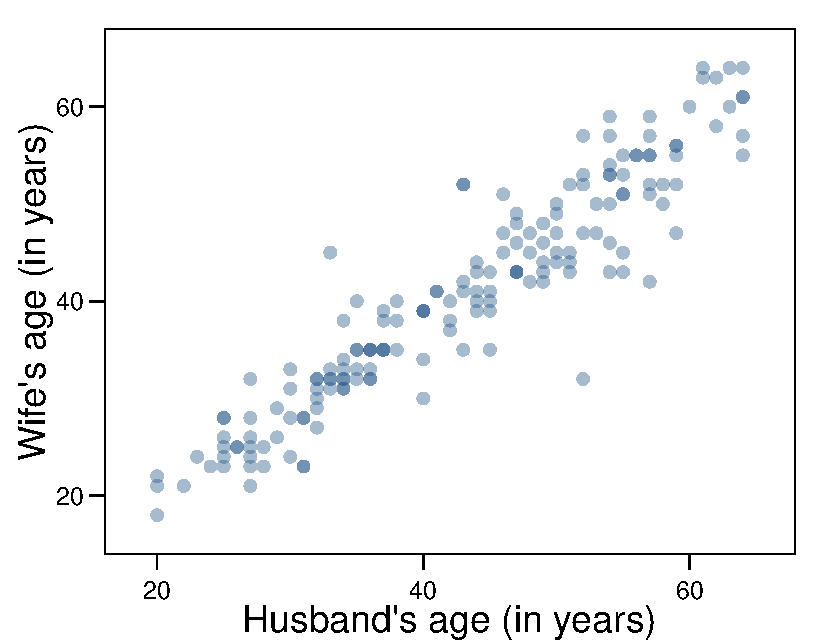
\includegraphics[width=0.45\textwidth]{07/figures/eoce/husbandsWivesAge.pdf}
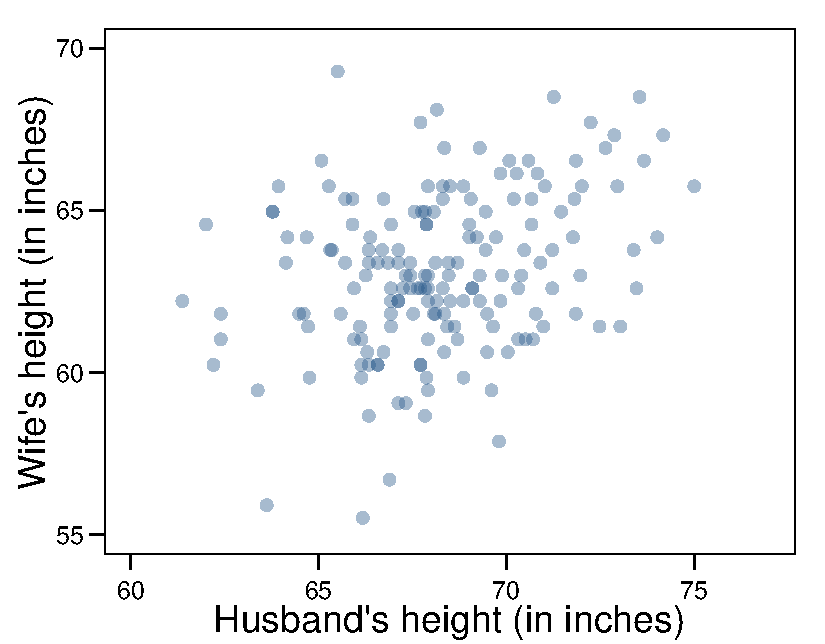
\includegraphics[width=0.45\textwidth]{07/figures/eoce/husbandsWivesHeight.pdf}
\end{center}
\begin{enumerate}[(a)]
\setlength{\itemsep}{0mm}
\item Describe the relationship between husbands' and wives' ages.
\item Describe the relationship between husbands' and wives' heights.
\item Which plot shows a stronger correlation? Explain your reasoning.
\item Data on heights were originally collected in centimeters, and then converted to inches. Does this conversion affect the correlation between husbands' and wives' heights?
\end{enumerate}
}
{
\begin{enumerate}[(a)]
\item The association between husbands' and wives' ages is positive, weak, and linear. There are two potential outliers: a 33 year old man married to a 45 year old woman, and a 52 year old man married to a 32 year old woman. 
\item The association between husbands' and wives' ages is positive, strong, and linear. Since there is a lot of scatter potential outliers are harder to pinpoint. However the 66 inch tall man married to a woman who is 69 inches appear to be an outlier.
\item There is much less scatter in the age plot therefore the relationship is much stronger.
\item The correlation between heights in inches and heights in centimeters is the same since unit conversions do not affect correlation. The correlation coefficient is a unit less measure.
\end{enumerate}
}\label{husbandsWives}
% note: data from fathom sample documents, DPH had a similar question but this is based on fathom data.

% 7

\noindent \begin{minipage}[c]{0.3\textwidth}
\eoce{Match the calculated correlations to the corresponding scatterplot.
\begin{enumerate}[(a)]
\setlength{\itemsep}{3mm}
\item $R = -0.73$
\item $R = 0.35$ 
\item $R = -0.02$
\item $R = 0.92$
\end{enumerate}
\vspace{1.75cm}
}
{
\begin{multicols}{4}
\begin{enumerate}[(a)]
\item $R = -0.73$ $\rightarrow$ (4)
\item $R = 0.35$ $\rightarrow$ (3)
\item $R = -0.02$ $\rightarrow$ (1)
\item $R = 0.92$ $\rightarrow$ (2)
\end{enumerate}
\end{multicols}
}
\end{minipage}
\begin{minipage}[c]{0.7\textwidth}
\begin{center}
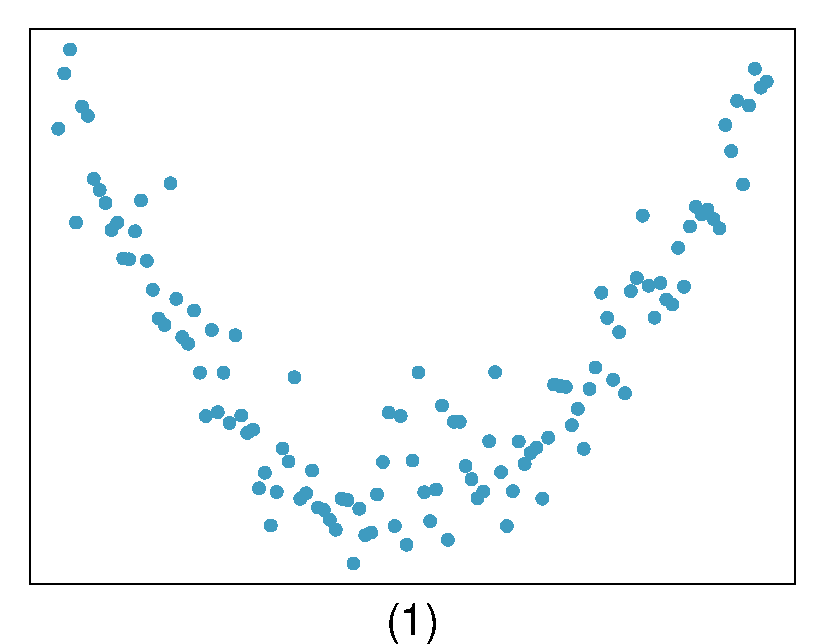
\includegraphics[width=0.45\textwidth]{07/figures/eoce/corrMatch1.pdf}
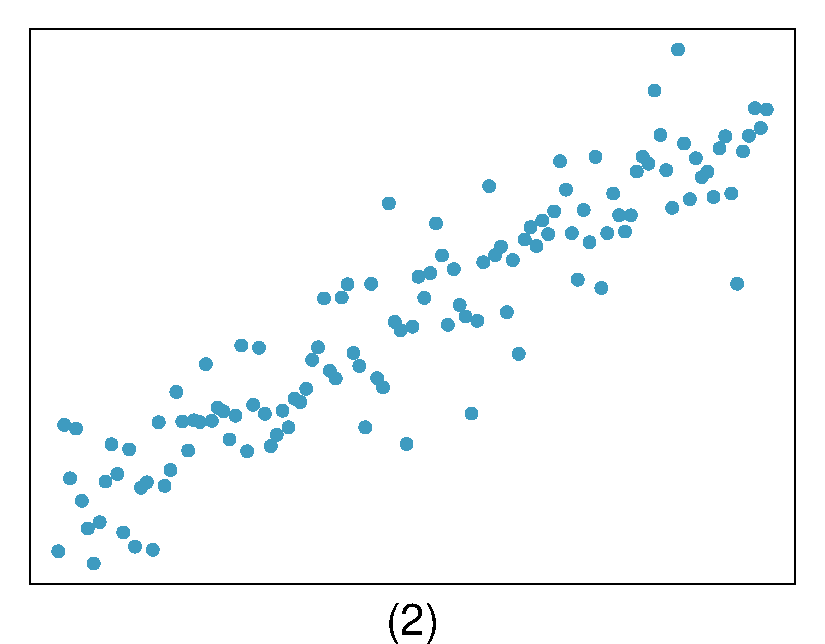
\includegraphics[width= 0.45\textwidth]{07/figures/eoce/corrMatch2.pdf} \\
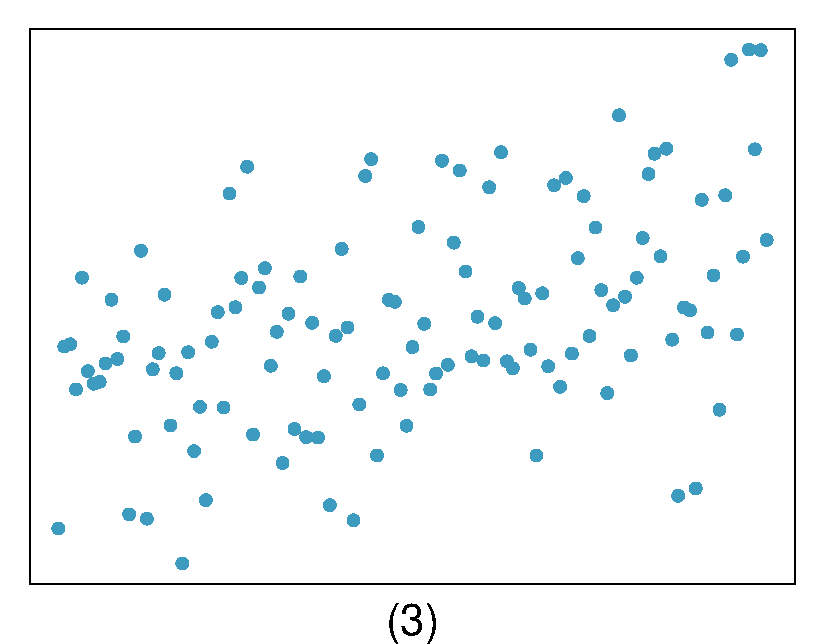
\includegraphics[width= 0.45\textwidth]{07/figures/eoce/corrMatch3.pdf}
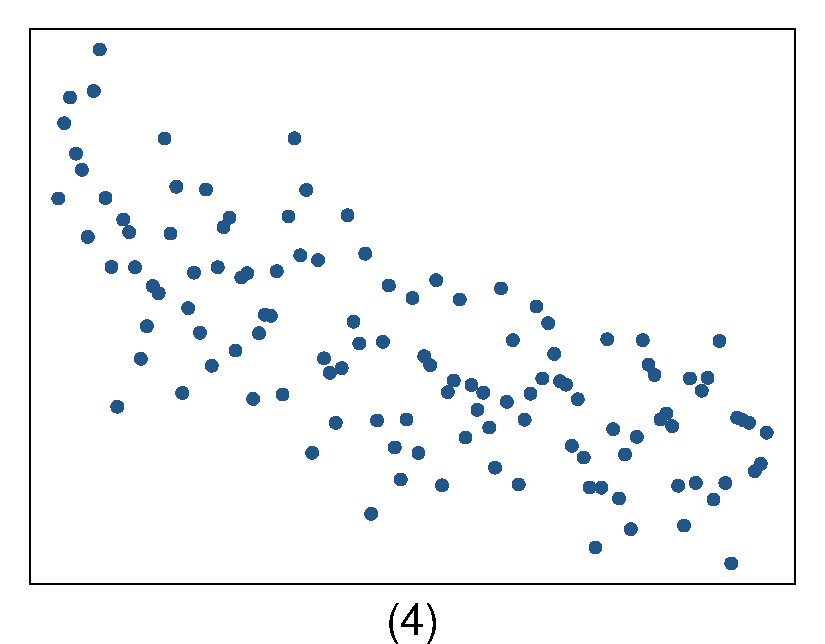
\includegraphics[width= 0.45\textwidth]{07/figures/eoce/corrMatch4.pdf}
\end{center}
\end{minipage}

% 8

\noindent \begin{minipage}[c]{0.3\textwidth}
\eoce{Match the calculated correlations to the corresponding scatterplot.
\begin{enumerate}[(a)]
\setlength{\itemsep}{3mm}
\item $R = 0.35$
\item $R = -0.52$ 
\item $R = -0.06$ 
\item $R = -0.80$
\end{enumerate}
\vspace{1.75cm}
}
{
\begin{multicols}{4}
\begin{enumerate}[(a)]
\item $R = 0.35$ $\rightarrow$ (2)
\item $R = -0.52$ $\rightarrow$ (4)
\item $R = -0.06$ $\rightarrow$ (3)
\item $R = -0.80$ $\rightarrow$ (1)
\end{enumerate}
\end{multicols}
}
\end{minipage}
\begin{minipage}[c]{0.7\textwidth}
\begin{center}
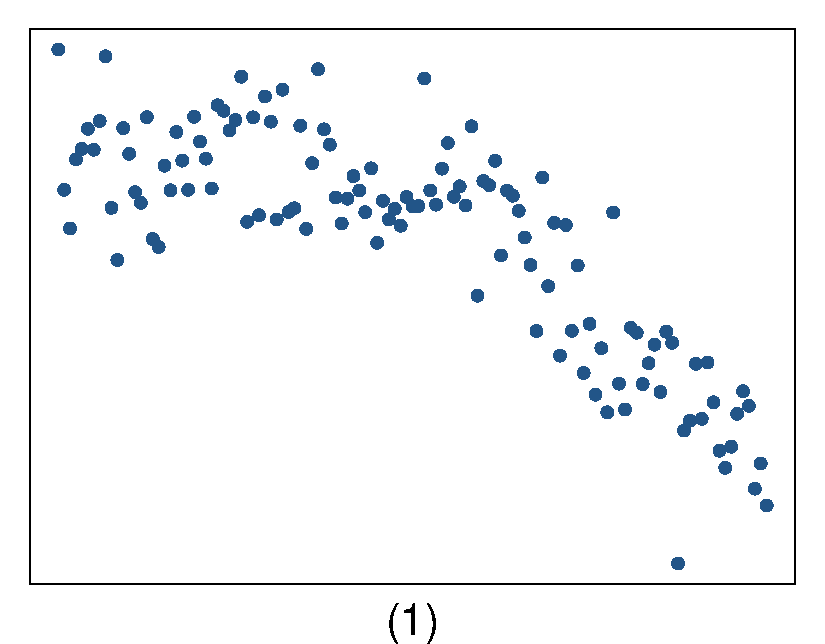
\includegraphics[width=0.45\textwidth]{07/figures/eoce/corrMatch5.pdf}
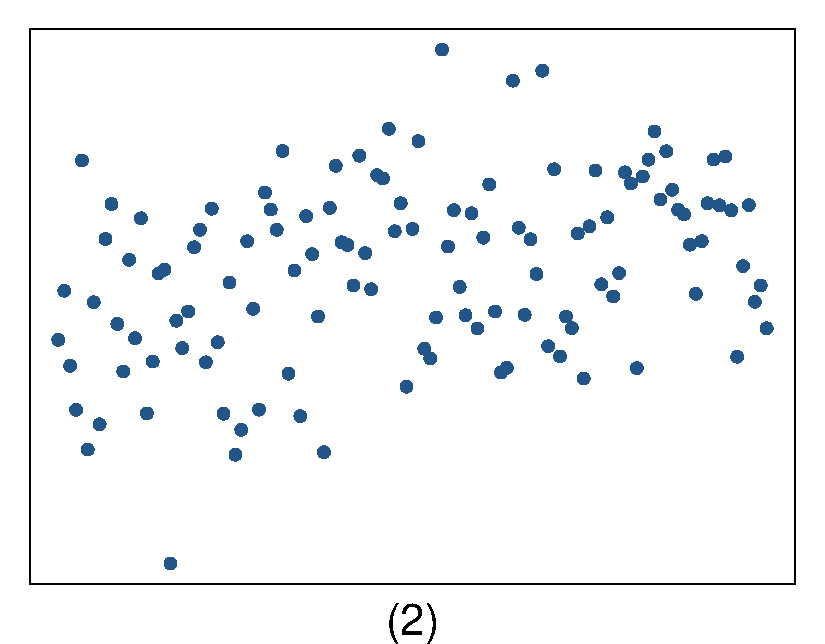
\includegraphics[width= 0.45\textwidth]{07/figures/eoce/corrMatch6.pdf} \\
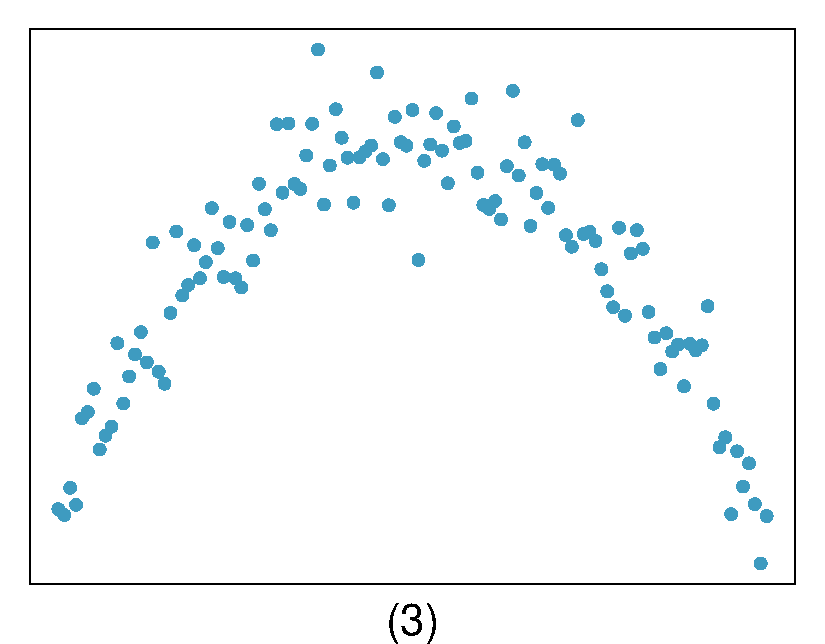
\includegraphics[width= 0.45\textwidth]{07/figures/eoce/corrMatch7.pdf}
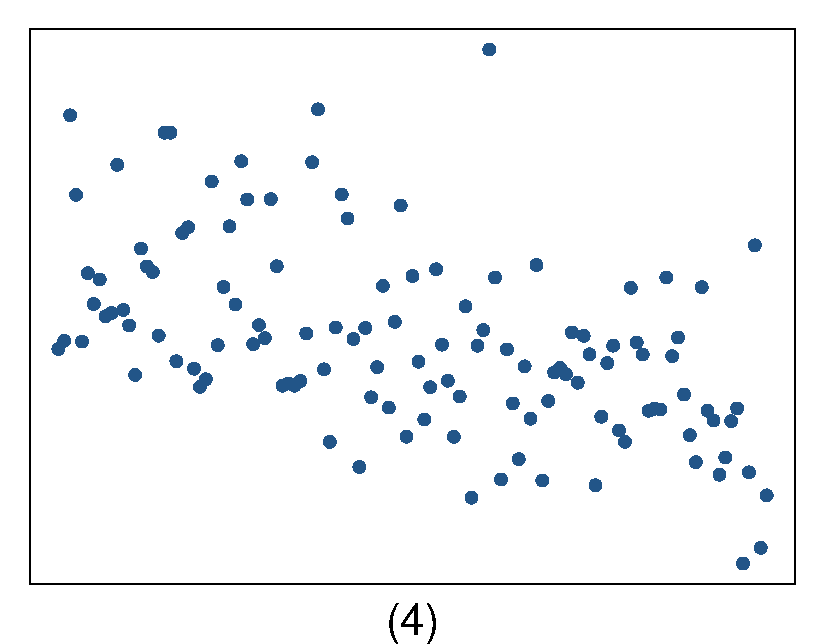
\includegraphics[width= 0.45\textwidth]{07/figures/eoce/corrMatch8.pdf}
\end{center}
\end{minipage}

% 9

\eoce{63 college students were asked to fill out a survey where they were asked about their height, fastest speed they ever drove at, and gender. Below is a scatterplot displaying the relationship between height and fastest speed.
\begin{center}
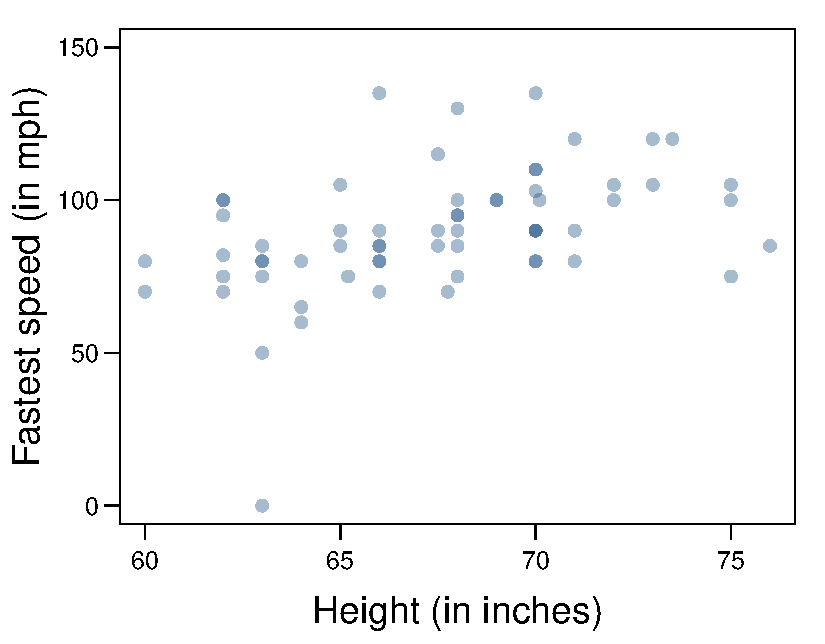
\includegraphics[width=0.6\textwidth]{07/figures/eoce/studentSurveySpeed.pdf}
\end{center}
\begin{enumerate}[(a)]
\setlength{\itemsep}{0mm}
\item Describe the relationship between height and fastest speed.
\item Why do you think these variables are positively associated?
\item Below is another scatterplot displaying the relationship between height and fastest speed. In this plot, female students are represented with triangles and male students are represented with circles. How does gender play a role in the relationship between height and fastest speed.
\end{enumerate}
\begin{center}
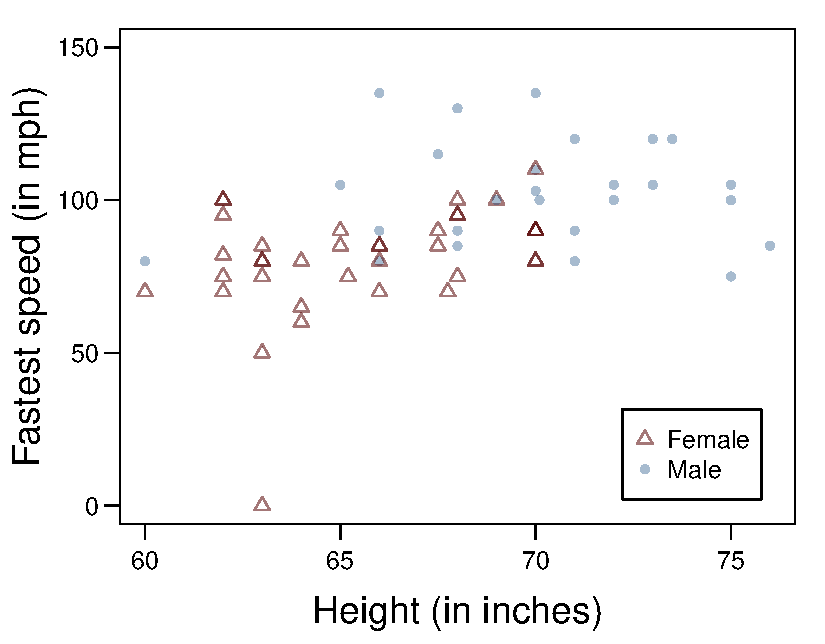
\includegraphics[width=0.65\textwidth]{07/figures/eoce/studentSurveySpeedGender.pdf}
\end{center}
}
{
\begin{enumerate}[(a)]
\item The relationship is positive, weak, and possibly linear. There appears to be one outlier, a student who is about 63 inches tall whose fastest speed is 0 mph. This is probably a student who doesn't drive.
\item There is no obvious explanation why simply being tall should lead a person to drive faster. However, one possible outside factor may be gender. Males tend to be taller than females on average, and and personal experiences (anecdotal) may suggest they drive faster (confirmed in sociological studies).
\item It appears that males are taller on average than females and they also drive faster. The gender variable is a lurking variable for the positive association we observe between fastest driving speed and height.
\end{enumerate}
}

% 10

\eoce{The scatterplots below show the relationship between height, diameter, and volume of timber in 31 felled black cherry trees. Note that the diameter of the tree is measured at 4 feet 6 inches above the ground. \citep{data:trees}
\begin{center}
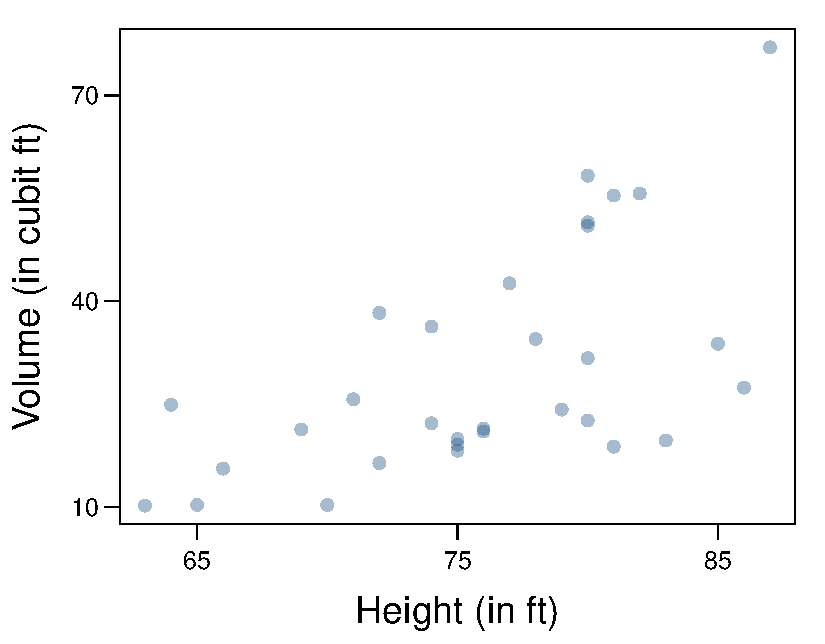
\includegraphics[width=0.495\textwidth]{07/figures/eoce/treesHeightVol}
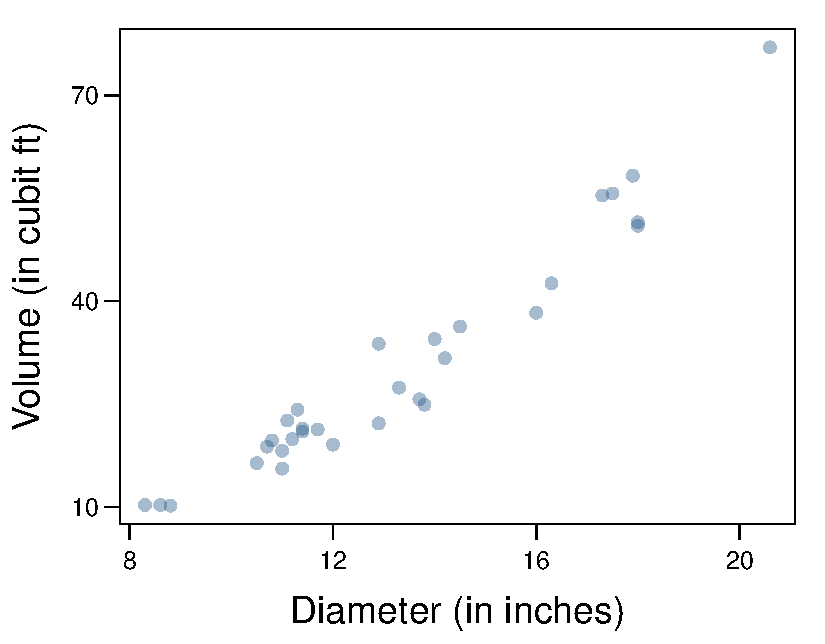
\includegraphics[width=0.495\textwidth]{07/figures/eoce/treesGirthVol}
\end{center}
\begin{enumerate}[(a)]
\setlength{\itemsep}{0mm}
\item Describe the relationship between volume and height of these trees.
\item Describe the relationship between volume and diameter of these trees.
\item Suppose you have height and diameter measurements for another black cherry tree. Which of these variables would you prefer to use to predict the volume of timber in this tree using a simple linear regression model? Explain your reasoning.
\end{enumerate}
}
{
\begin{enumerate}[(a)]
\setlength{\itemsep}{0mm}
\item There is a moderately strong, positive, linear association between height and volume. There also appears to be some non-constant variance since the volume of trees is more variable for taller trees.
\item There is a very strong, positive association between diameter and volume. However it is difficult to tell if this relationship is linear or somewhat curved. We would need to see a residuals plot to determine the form of the relationship.
\item Since the relationship is stronger between volume and diameter, using diameter would be preferred. However, as mentioned in part (b), the relationship between volume and diameter may not be linear.
\end{enumerate}
}


\pagebreak
% 11

\eoce{The Coast Starlight Amtrak train runs from Seattle to Los Angeles. The scatterplot below displays the distance between each stop (in miles) and the amount of time it takes to travel from one stop to another (in minutes).
\begin{multicols}{2}
\begin{enumerate}[(a)]
\setlength{\itemsep}{0mm}
\item Describe the relationship between distance and travel time.
\item How would the relationship change if travel time was instead measured in hours, and distance was instead measured in kilometers?
\item Correlation between travel time (in miles) and distance (in minutes) is $R = 0.636$. What is the correlation between travel time (in kilometers) and distance (in hours).
\end{enumerate}
%\begin{center}
\includegraphics[width=0.5\textwidth]{07/figures/eoce/coastStarScat.pdf}
%\end{center}
\end{multicols}
}
{
\begin{enumerate}[(a)]
\item There is a somewhat weak, positive, possibly linear relationship between the distance traveled and travel time.
\item Changing the units will not change the form, direction or strength of the relationship between the two variables. After all if longer distances measured in miles are associated with longer travel time measured in minutes, longer distances measured in kilometers will be associated with longer travel time measured in hours.
\item Since changing units doesn't affect correlation, $R = 0.636$.
\end{enumerate}
}\label{coastStarlight}

% 12

\eoce{A study conducted at University of Denver investigated whether babies take longer to learn to crawl in cold months, when they are often bundled in clothes that restrict their movement, than in warmer months \citep{Benson:1993}. Infants born during the study year were split into twelve groups, one for each birth month. We consider the average crawling age of babies in each group against the average temperature when the babies are six months old (that's when babies often begin trying to crawl). Temperature is measured in degrees Fahrenheit (\degree F) and age is measured in weeks.
\begin{center}
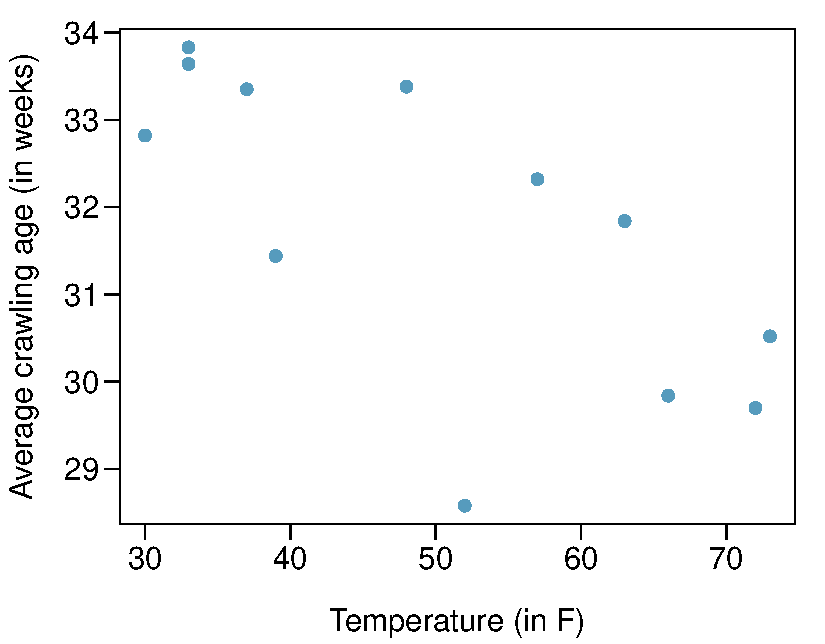
\includegraphics[width=0.6\textwidth]{07/figures/eoce/babiesCrawl}
\end{center}
\begin{enumerate}[(a)]
\item Describe the relationship between temperature and crawling age.
\item How would the relationship change if temperature was measured in degrees Celsius (\degree C) and age was measured in months instead of in weeks?
\item The correlation between temperature in Fahrenheit and age in weeks was $R=-0.70$. If we converted the temperature to Celsius and age to months, what would the correlation be?
\end{enumerate}
}
{
\begin{enumerate}[(a)]
\item The relationship is somewhat strong, negative, and linear. There is also an outlying month when the average temperature is about 53\degree F and average crawling age is about 28.5 weeks.
\item Changing the units will not change the form, direction or strength of the relationship between the two variables. After all, if higher temperatures measured in \degree F are associated with lower average crawling age measured in weeks, higher temperatures measured in \degree C will be associated with lower average crawling age measured in months.
\item Since changing units doesn't affect correlation, $R = -0.70$.
\end{enumerate}
}\label{babiesCrawl}

% 13

{\eoce{Researchers studying anthropometry collected body girth measurements and skeletal diameter measurements, as well as age, weight, height and gender for 507 physically active individuals \citep{Heinz:2003}. The scatterplot below shows the relationship between height and shoulder girth (over deltoid muscles), both measured in centimeters.
%\begin{multicols}{2}
\begin{enumerate}[(a)]
%\item[]
\item Describe the relationship between shoulder girth and height.
\item How would the relationship change if shoulder girth was measured in inches while the units of height remained in centimeters?
%\item[]
%\item[]
\end{enumerate}
\begin{center}
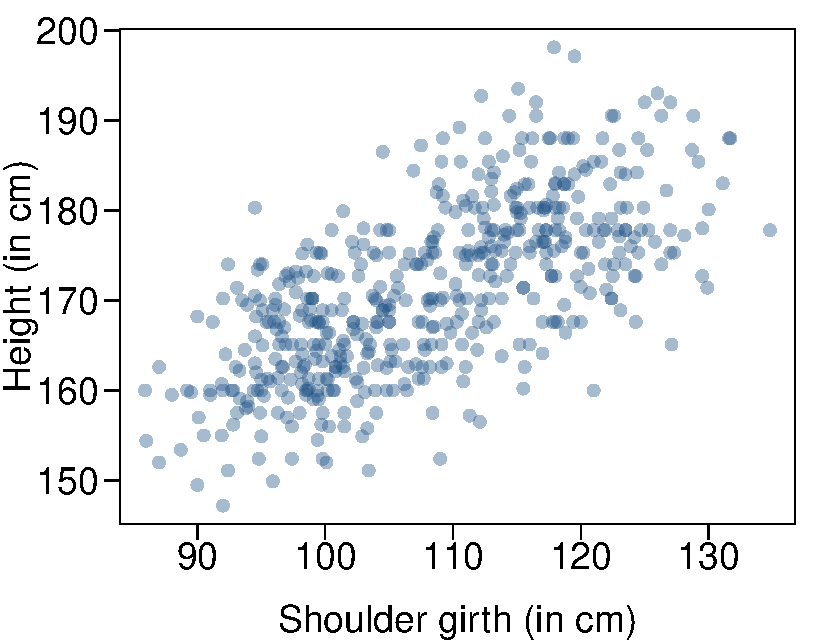
\includegraphics[width=0.6\textwidth]{07/figures/eoce/bodyHgtShoGi}
\end{center}
%\end{multicols}
}
{
\begin{enumerate}[(a)]
\item There is a moderately strong, positive, linear relationship between shoulder girth and height.
\item Changing the units, even if just for one of the variables, will not change the form, direction or strength of the relationship between the two variables.
\end{enumerate}
}\label{bodyHgtShoGi}
}

% 14

\eoce{The scatterplot below shows the relationship between weight measured in kilograms and hip girth measured in centimeters from the data described in Exercise~\eoceref{bodyHgtShoGi}.
\begin{multicols}{2}
\begin{enumerate}[(a)]
\setlength{\itemsep}{0mm}
\item[]
\item Describe the relationship between hip girth and weight.
\item How would the relationship change if weight was measured in pounds while the units for hip girth remained in centimeters?
\item[]
\end{enumerate}
\begin{center}
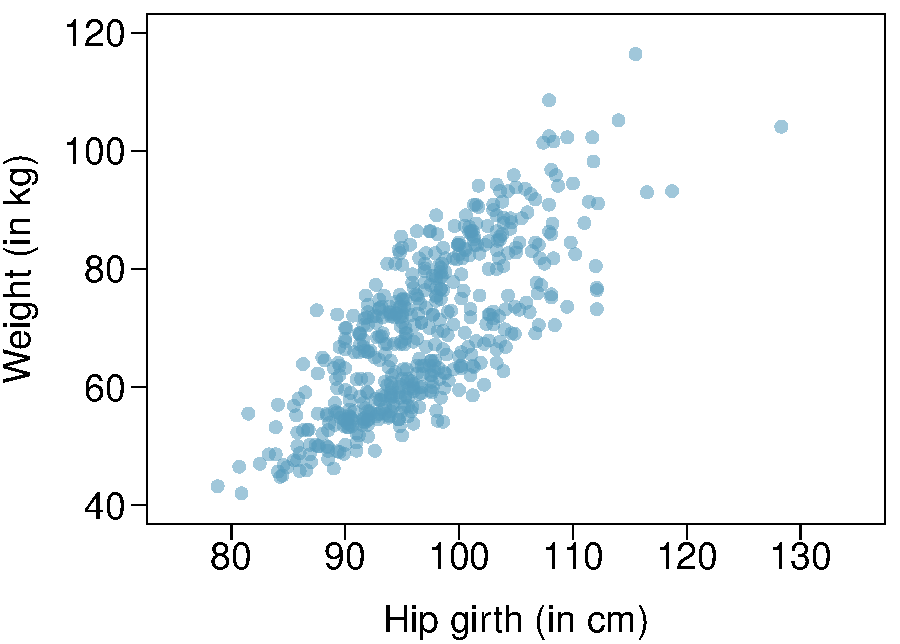
\includegraphics[width=0.5\textwidth]{07/figures/eoce/bodyWgtHipGi}
\end{center}
\end{multicols}
}
{
\begin{enumerate}[(a)]
\item The relationship is strong and positive. However there appears to be some departure from linearity as the scatterplot shows somewhat of a fan shape. There is less variability in weights for people with lower hip girth measurements than for people with larger hip girth measurements. One explanation for the fan shape might be that the data are composed of two groups of people (males and females) who are likely to have a different relationship between their weights and hip girths.
\item Changing the units, even if just for one of the variables, will not change the form, direction or strength of the relationship between the two variables.
\end{enumerate}
}\label{bodyWgtHipGi}

% 15

\eoce{What would be the correlation between the ages of husbands and wives if men always married woman who were
\begin{enumerate}[(a)]
\setlength{\itemsep}{0mm}
\item 3 years younger than themselves? 
\item 2 years older than themselves? 
\item half as old as themselves?
\end{enumerate}
}
{
The simplest way to answer these questions is to simulate a data set.
\begin{enumerate}[(a)]
\item Let's assume we have three men ages 30, 31 and 32. Then, their wives will be 27, 28 and 29. There is a one-to-one relationship between the ages of husbands of wives, therefore $R = 1$.
\item Assuming once again that we have three men ages 30, 31 and 32, their wives will be 32, 33 and 34. There is a one-to-one relationship between the ages of husbands of wives, therefore $R = 1$.
\item This time let's assume we have three men aged 60, 61 and 62. Then, their wives will be 30, 30.5 and 31. Once again there is a one-to-one relationship between the ages of husbands of wives, therefore $R = 1$.
\end{enumerate}
\begin{center}
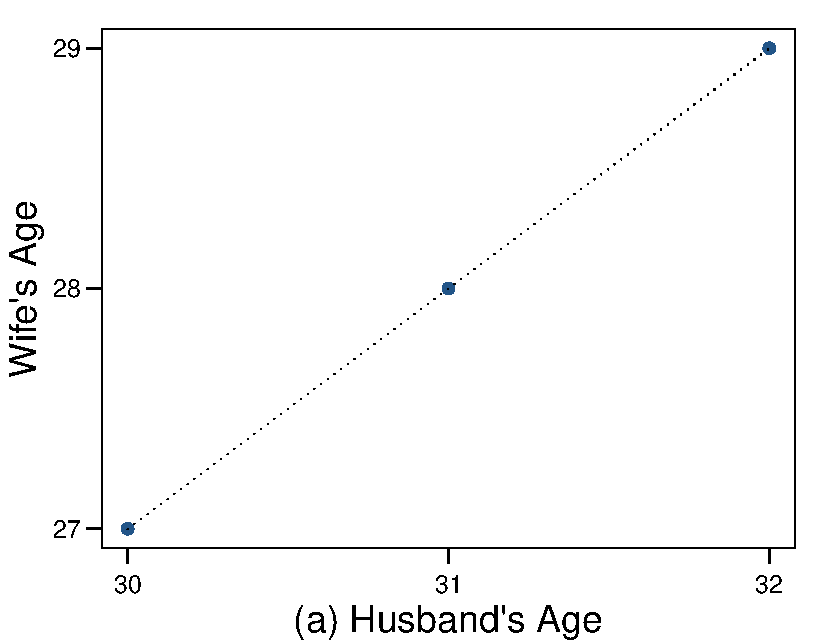
\includegraphics[width=49mm]{07/figures/eoce/husWifeA.pdf}
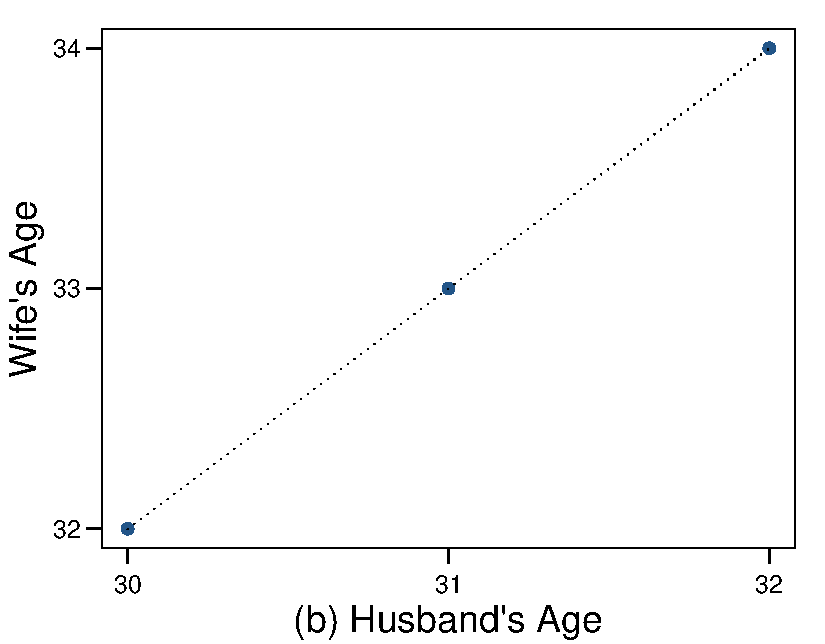
\includegraphics[width=49mm]{07/figures/eoce/husWifeB.pdf}
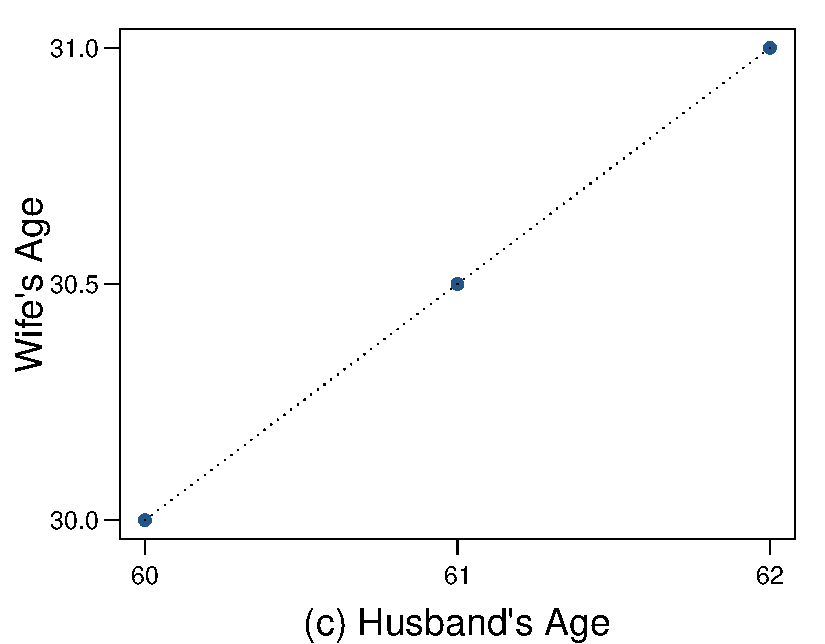
\includegraphics[width=49mm]{07/figures/eoce/husWifeC.pdf}
\end{center}
}

% 16

\eoce{What would be the correlation between the annual salaries of males and females at a company if for a certain type of position men always made
\begin{enumerate}[(a)]
\item \$5,000 more than women?
\item 25\% more than women?
\item 15\% less than women?
\end{enumerate}
}
{
The simplest way to answer these questions is to simulate a data set.
\begin{enumerate}[(a)]
\item Let's assume we have three men with salaries \$20,000, \$30,000, and \$40,000. Then women who have similar positions will make \$15,000, \$25,000, and \$35,000. There is a one-to-one relationship between the salaries of these men and women, therefore $R = 1$.
\item Assuming once again that we have three men with salaries \$20,000, \$30,000, and \$40,000, women who have similar positions will make \$20,000 / 1.25 = \$16,000, \$30,000 / 1.25 = \$24,000, and \$40,000 / 1.25 = \$32,000. There is a one-to-one relationship between the salaries of these men and women, therefore $R = 1$.
\item Assuming once again that we have three men with salaries \$20,000, \$30,000, and \$40,000, women who have similar positions will make \$20,000 / 0.85 = \$23,529.41, \$30,000 / 0.85 = \$24,000, and \$40,000 / 0.85 = \$47058.82. There is a one-to-one relationship between the salaries of these men and women, therefore $R = 1$.
\end{enumerate}
\begin{center}
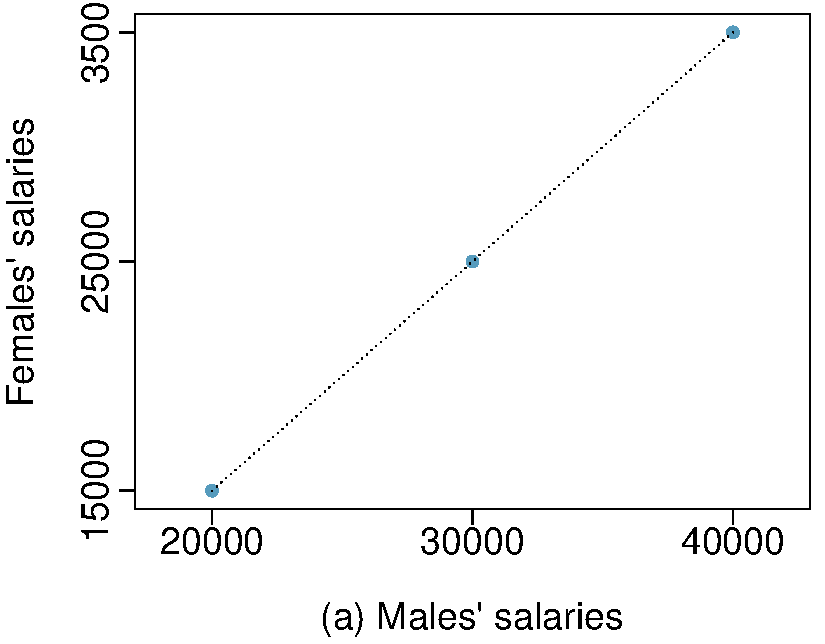
\includegraphics[width=49mm]{07/figures/eoce/mfSalA}
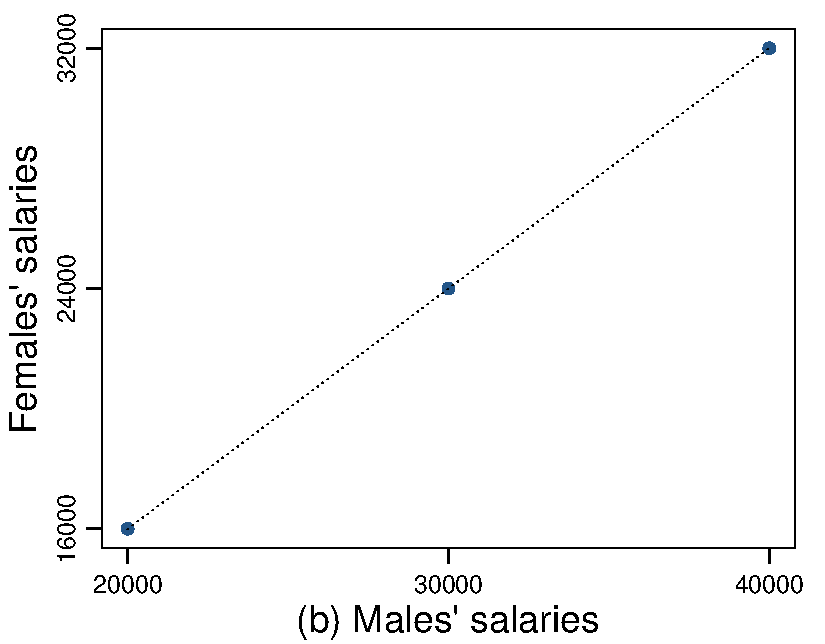
\includegraphics[width=49mm]{07/figures/eoce/mfSalB}
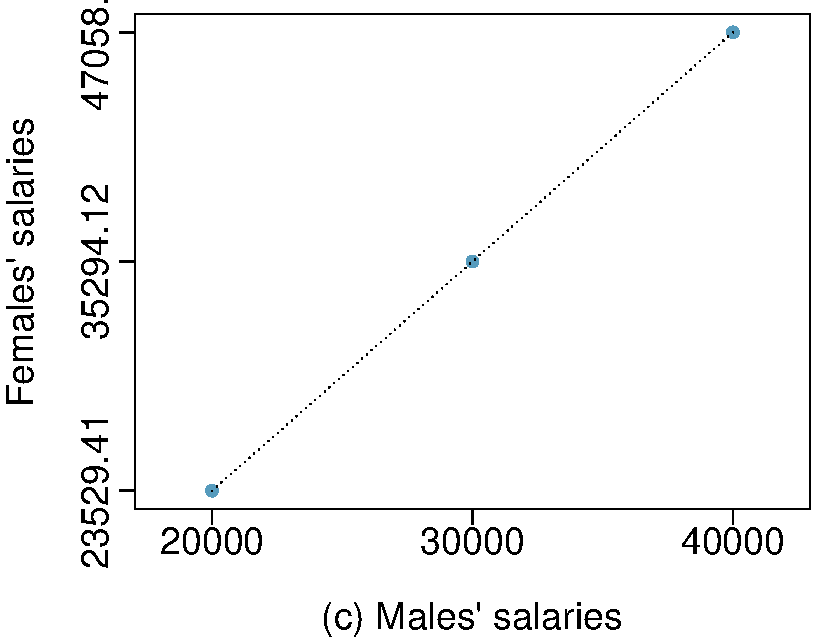
\includegraphics[width=49mm]{07/figures/eoce/mfSalC}
\end{center}
}

%%%%%%%%%%%%%%%%%%%%%

\subsection{Fitting a line by least squares regression}

%%%%%%%%%%%%%%%%%%%%%

% 17

\eoce{The Association of Turkish Travel Agencies reports the number of foreign tourists visiting Turkey and tourist spending by year \citep{data:turkeyTourism}. The  scatterplot below shows the relationship between these two variables along with the least squares fit. \vspace{-5mm}
\begin{multicols}{2}
\begin{enumerate}[(a)]
\item[]
\item Describe the relationship between number of tourists and spending.
\item What are the explanatory and response variables?
\item Why might we want to fit a regression line to these data?
\item[]
\end{enumerate}
\begin{center}
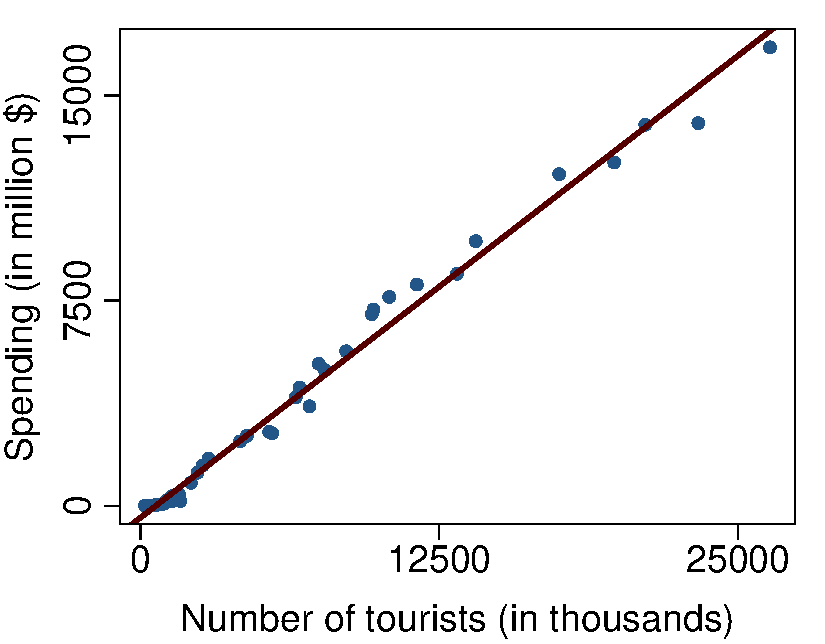
\includegraphics[width=0.5\textwidth]{07/figures/eoce/turkeyTourismScat.pdf}
\end{center}
\end{multicols}
}
{
\begin{enumerate}[(a)]
\item There is a positive, very strong, linear association between number of tourists and spending. 
\item Explanatory variable is number of tourists (in thousands) and response variable is spending (in million \$).
\item We can predict spending for a given number of tourists using a regression line. This may be useful information for determining how much the country may want to spend in advertising abroad, or to forecast expected revenues from tourism.
\end{enumerate}
}\label{turkeyTourism}

% 18

\eoce{The scatterplot below shows the relationship between number of calories and amount of carbohydrates (in grams) Starbucks food menu items contain \citep{data:starbucksCals}. Since Starbucks only lists the number of calories on the display items, we are interested in predicting the amount of carbs a menu item has based on its calorie content.
\begin{multicols}{2}
\begin{enumerate}[(a)]
\item Describe the relationship between number of calories and amount of carbohydrates (in grams) Starbucks food menu items contain.
\item In this scenario, what are the explanatory and response variables?
\item Why might we want to fit a regression line to these data?
\end{enumerate}
\begin{center}
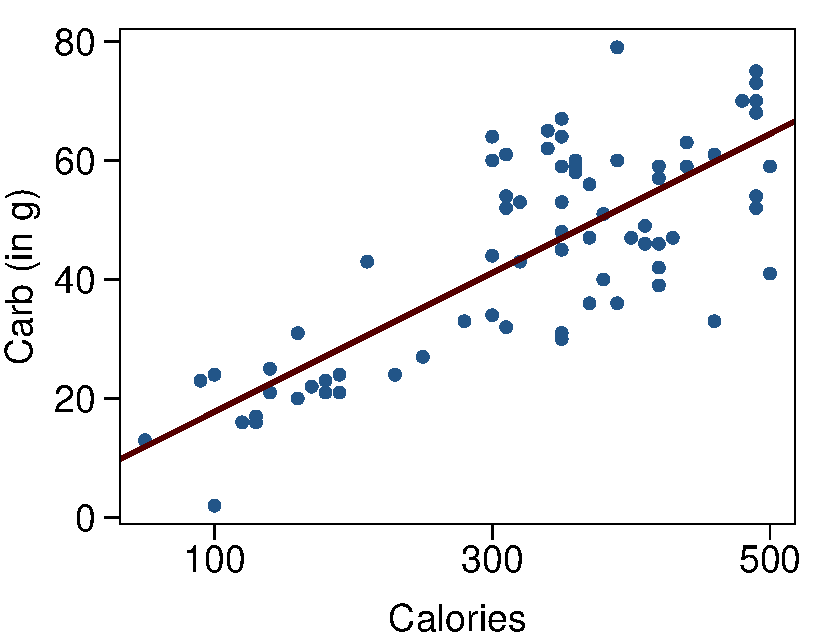
\includegraphics[width=0.5\textwidth]{07/figures/eoce/starbucksCarbCals.pdf}
\end{center}
\end{multicols}
}
{
\begin{enumerate}[(a)]
\item There is a positive, moderately strong, linear association between number of calories and amount of carbohydrates. In addition, the amount of carbohydrates is more variable for menu items with higher calories, indicating non-constant variance.
\item Explanatory variable is number of calories and response variable is amount of carbohydrates (in grams).
\item With a regression line we can predict the amount of carbohydrates for a given number of calories. This may be useful information if only calorie counts for the food items are posted but the amount of carbohydrates is not readily available.
\end{enumerate}
}\label{starbucksCarbCals}

\pagebreak
% 19

\eoce{Does the tourism data plotted in Exercise~\eoceref{turkeyTourism} meet the conditions required for fitting a least squares line? In addition to the scatterplot provided in Exercise~\eoceref{turkeyTourism}, use the residuals plot and the histogram below to answer this question. 
\begin{center}
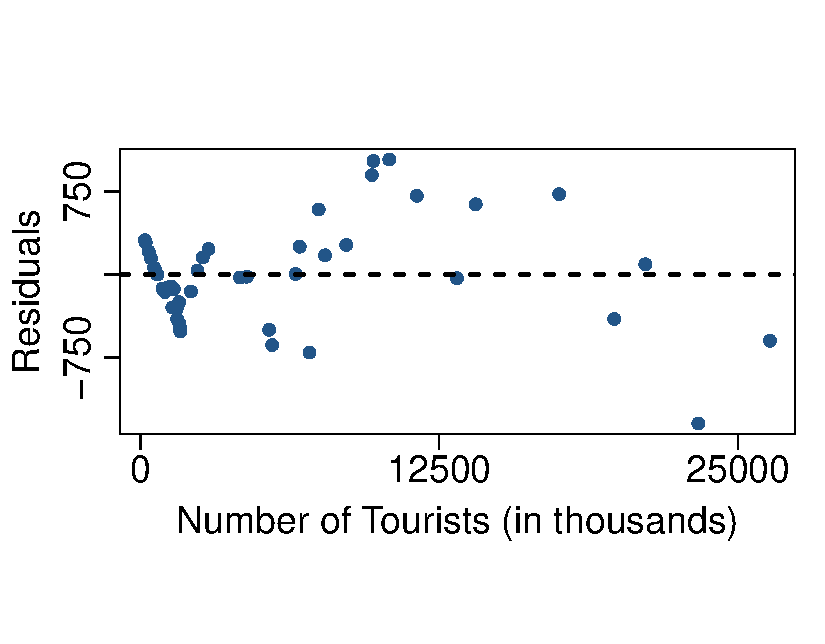
\includegraphics[width=0.45\textwidth]{07/figures/eoce/turkeyTourismResScat.pdf}
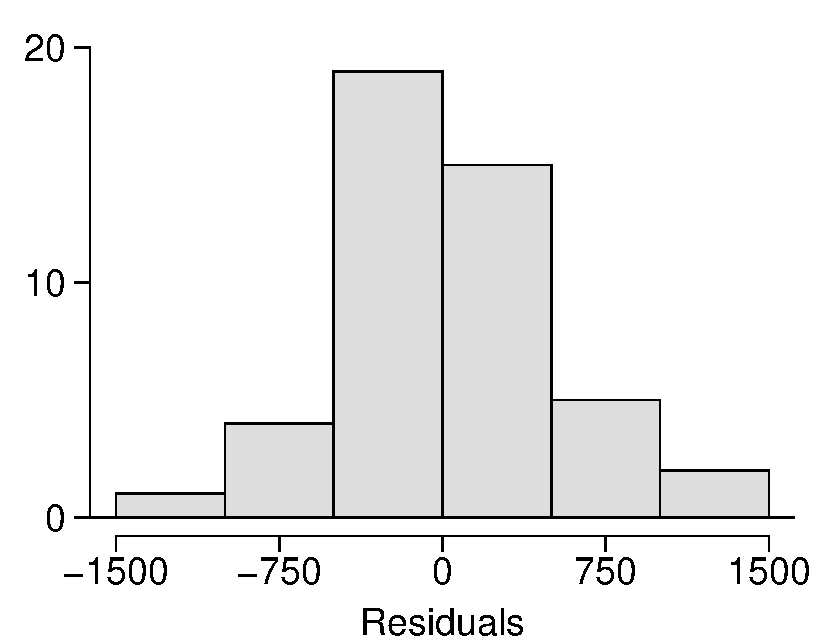
\includegraphics[width=0.45\textwidth]{07/figures/eoce/turkeyTourismResHist.pdf}
\end{center}
}
{
Even though the relationship appears linear in the scatterplot, the residuals plot actually shows a non-linear relationship. This is not a contradiction, residual plots can show any slight divergences from linearity that can be hidden in scatterplots. It is difficult to tell from the residuals plot if the residuals have a constant variance due to the curved shape. From the histogram we can see that the residuals are distributed approximately normally. However since the relationship is not linear, we do not need to check the other two conditions (nearly normal residuals and constant variability) as violation of one condition is sufficient to determine that we should not fit a least squares line to this data.
}

% 20

\eoce{Does the Starbucks nutrition data plotted in Exercise~\eoceref{starbucksCarbCals} meet the conditions required for fitting a least squares line? In addition to the scatterplot provided in Exercise~\eoceref{starbucksCarbCals}, use the residuals plot and the histogram below to answer this question. 
\begin{center}
\includegraphics[width= 0.45\textwidth]{07/figures/eoce/starbucksCarbCalsResScat.pdf}
\includegraphics[width= 0.45\textwidth]{07/figures/eoce/starbucksCarbCalsResHist.pdf}
\end{center}
}
{
Even though the relationship appears linear in the scatterplot, there is some possible structure remaining in the residuals, either a fan shape or curvature. Both of these suggest that there may be a nonlinear relationship between calorie and carb content of the menu items. From the histogram we can see that the residuals are distributed approximately normally. However since the constant variability assumption is violated we should not fit a least squares line to this data.
}


% 21

\eoce{Exercise~\eoceref{coastStarlight} introduces data on the Coast Starlight Amtrak train that runs from Seattle to Los Angeles. The mean travel time from one stop to the next on the Coast Starlight is 129 mins, with a standard deviation of 113 minutes. The mean distance traveled from one stop to the next is 107 miles with a standard deviation of 99 miles. The correlation between travel time and distance is 0.636.
\begin{enumerate}[(a)]
\setlength{\itemsep}{0mm}
\item Write the equation of the regression line for predicting travel time.
\item Interpret the slope and the intercept in context.
\item The distance between Santa Barbara and Los Angeles is 103 miles. Use the model to estimate the time it takes for the Starlight to travel between these two cities.
\item It actually takes the the Coast Starlight 168 mins to travel from Santa Barbara to Los Angeles. Calculate the residual and explain the meaning of this residual value.
\item Suppose Amtrak is considering adding a stop to the Coast Starlight 500 miles away from Los Angeles. Would it be appropriate to use this linear model to predict the travel time from Los Angeles to this point? 
\end{enumerate}
}
{
\begin{enumerate}[(a)]
\item First we calculate the slope.
\[ b_1 = \frac{s_y}{s_x} R = \frac{113}{99} \times 0.636 = 0.726 \]
Then we make use of the fact that the regression line passes through the point $(\bar{x},\bar{y})$.
\begin{align*}
\bar{y} &= b_0 + b_1 \times \bar{x} \\
129 &= b_0 + 0.726 \times 107 \\
b_0 &=  129 - 0.726 \times 107 = 51 \\
\end{align*}
The regression line can be written as
\[ \widehat{travel~time} = 51 + 0.726 \times distance \]
\item $b_1$ = For each additional mile in distance, the model predicts an additional 0.726 minutes in travel time. \\
$b_0$ = When the distance traveled is 0 miles, the travel time is expected to be 51 minutes. It does not make sense to have a travel distance of 0 miles. Here, the $y$-intercept serves only to adjust the height of the line and is meaningless by itself.
\item In order to calculate the predicted time it takes to travel from Santa Barbara to Los Angeles we plug in 103 for distance in the model:
\[ \widehat{travel~time} =  51 + 0.726 \times distance = 51 + 0.726 \times 103 \approx 126~minutes \]
\item The residual can be calculated as $e_i = y_i - \hat{y}_i = 168 - 126 = 42$ minutes. A positive residual means that the model underestimates the travel time.
\item No, we should not use this linear model to predict the travel time for a distance of 500 miles as this would be extrapolation. The data we used to create the model is for approximately 10 to 350 miles of distance. The linear model may no longer hold outside the range of the data.
\end{enumerate}
}\label{coastStarlightReg}


% 22

\eoce{Exercise~\eoceref{bodyHgtShoGi} introduces data on shoulder girth and height of a group of individuals. The mean shoulder girth is 108.20 cm with a standard deviation of 10.37 cm. The mean height is 171.14 cm with a standard deviation of 9.41 cm. The correlation between height and shoulder girth is 0.666.
\begin{enumerate}[(a)]
\setlength{\itemsep}{0mm}
\item Write the equation of the regression line for predicting height.
\item Interpret the slope and the intercept in context.
\item A randomly selected student from your class has a shoulder girth of 100 cm. Predict the height of this student.
\item This student is actually 160 cm tall. Calculate the residual and explain what this residual means.
\item A one year old has a shoulder girth of 56 cm. Would it be appropriate to use this linear model to predict the height of this child?
\end{enumerate}
}
{
\begin{enumerate}[(a)]
\item First we calculate the slope.
\[ b_1 = \frac{s_y}{s_x} R = \frac{9.41}{10.37} \times 0.666 = 0.604\]
Then we make use of the fact that the regression line passes through the point $(\bar{x},\bar{y})$.
\begin{align*}
\bar{y} &= b_0 + b_1 \bar{x}) \\
171.14 &= b_0 + 0.604 \times 108.20 \\
b_0 &=  0.604 \times 108.20 - 171.14
\end{align*}
The regression line can be written as
\[ \widehat{height} =  105.79 + 0.604 \times shoulderGirth \]
\item $b_1$ = For each centimeter increase in shoulder girth we would expect height to increase on average by 0.604 centimeters. \\
$b_0$ = People who have a shoulder girth of 0 cm are expected on average to be 105.79 cm tall. A person with a 0 cm shoulder girth does not make any sense. Here, the $y$-intercept serves only to adjust the height of the line and is meaningless by itself.
\item In order to calculate height from shoulder girth we plug in 100 for shoulder girth in the model:
\[ \widehat{height} =  105.79 + 0.604 \times shoulderGirth = 105.79 + 0.604 \times 100 \approx 166~cm \]
\item The residual can be calculated as $e_i = y_i - \hat{y}_i = 160 - 166 = -6$ cm. A negative residual means that the model overestimates this student's height.
\item No, we should not use this linear model to predict the height of this child as this would be extrapolation. The data used to create the model is for people with approximately 90 to 130 cm shoulder girth. The linear model may no longer hold outside the range of the data.
\end{enumerate}
}\label{bodyHgtShoGiReg}

% 23

\eoce{Based on the information given in Exercise~\eoceref{coastStarlightReg}, calculate $R^2$ of the regression line for predicting travel time from distance traveled for the Coast Starlight and interpret it in context.}
{
$R^2 = 0.636^2 = 0.40$. \\
Approximately 40\% of the variability in travel time is accounted for by the model, i.e. explained by distance traveled.
}

% 24

\eoce{Based on the information given in Exercise~\eoceref{bodyHgtShoGiReg}, calculate $R^2$ of the regression line for predicting height from shoulder girth and interpret it in context.}
{
$R^2 = 0.666^2 = 0.44$. \\
Approximately 44\% of the variation in heights is accounted for by the model, i.e. explained by shoulder girth.
}

% 25

\noindent \begin{minipage}[c]{0.55\textwidth}
\eoce{
Data were collected on the number of hours per week students watch TV and the grade they earned in a statistics class (out of 100). Based on the scatterplot and the residuals plot provided, describe the relationship between the two variables and determine if a simple linear model is appropriate to predict grade from the number of hours per week the student watches TV.
\vspace{2.5cm}
}
{
The relationship appears to be linear, negative and strong. However there appears to be two outliers, the student who did not watch any TV but got a 82 in the class and the student who watched 32 hours of TV and got an 85 in the class. The latter seems to have a substantial pull on the line; therefore, a linear model may not be appropriate for these data. The residuals does not show a random scatter around 0, which further suggests that a linear model may not be appropriate.}
\end{minipage}
\begin{minipage}[c]{0.43\textwidth}
\begin{center}
\includegraphics[width= 0.85\textwidth]{07/figures/eoce/gradesTV.pdf} \\
\includegraphics[width= 0.85\textwidth]{07/figures/eoce/gradesTVRes.pdf}
\end{center}
\end{minipage}

% 26

\noindent \begin{minipage}[c]{0.55\textwidth}
\eoce{
Exercise~\eoceref{starbucksCarbCals} introduces a data set on nutrition information on Starbucks food menu items. Based on the scatterplot and the residuals plot provided, describe the relationship between the protein content and calories of these menu items and determine if a simple linear model is appropriate to predict protein amount from the number of calories.
\vspace{2.5cm}
}
{
There is a positive relationship between protein amount and calories however the relationship has non-constant variance. The variability in the protein amount of menu items with lower calories is much lower than that of menu items with higher calories. This is indicated by the fan shaped scatterplot as well as the fan shaped residuals plot. Since the constant variance assumption is not met, a linear model is not appropriate for these data. It should also be noted that there are three apparent outliers (menu items with about 400 calories and more than 25 grams of protein), two of which are not easily identifiable on the residual plot.
}
\end{minipage}
\begin{minipage}[c]{0.43\textwidth}
\begin{center}
\includegraphics[width= 0.85\textwidth]{07/figures/eoce/starbucksProCals.pdf} \\
\includegraphics[width= 0.85\textwidth]{07/figures/eoce/starbucksProCalsRes.pdf}
\end{center}
\end{minipage}

%%%%%%%%%%%%%%%%%%%%%

\subsection{Types of outliers in linear regression}

%%%%%%%%%%%%%%%%%%%%%

% 27

\eoce{Identify the outliers in the scatterplots shown below and determine what type of outliers they are. Explain your reasoning.
\begin{center}
\includegraphics[width=45mm]{07/figures/eoce/outInf1.pdf}
\includegraphics[width=45mm]{07/figures/eoce/outLev1.pdf}
\includegraphics[width=45mm]{07/figures/eoce/outOut1.pdf}
\end{center}
}
{
\begin{enumerate}[(a)]
\item The outlier is located in the bottom right corner of the plot away from the regression line. It is an influential point since if we were to exclude this point from the analysis the slope of the regression line would be affected greatly.
\item The outlier is located in the bottom right corner of the plot on the regression line. It is a leverage point since it is horizontally away from the center of the data but is not influential as it is on the trajectory of the regression line.
\item The outlier is located in the center of the top of the plot. It is neither an influential point not a leverage point. Though the point is unlike the rest of the data, it is not a leverage point as it is not far  on the $x$-axis from the center of the data and is not influential.
\end{enumerate}
}

% 28

\eoce{Identify the outliers in the scatterplots shown below and determine what type of outliers they are. Explain your reasoning.
\begin{center}
\includegraphics[width=45mm]{07/figures/eoce/outInf2.pdf}
\includegraphics[width=45mm]{07/figures/eoce/outInf3.pdf}
\includegraphics[width=45mm]{07/figures/eoce/outOut2.pdf}
\end{center}
}
{
\begin{enumerate}[(a)]
\item The outlier is located in the top left corner of the plot away from the regression line. It is an influential point since if we were to exclude this point from the analysis the slope of the regression line would be affected greatly.
\item The outlier is located in the bottom left corner of the plot away from the regression line. It is by definition an influential point but it does not appear to influence the regression line by much, but it has high leverage.
\item The outlier is located in the center of the top of the plot. Though the point is unlike the rest of the data, it is not a leverage point as it is not far  on the $x$-axis from the center of the data and is not influential.
\end{enumerate}
}

% 29

{
\eoce{Exercise~\eoceref{babiesCrawl} introduces data on the average monthly temperature during the month babies first try to crawl (about 6 months after birth) and the average first crawling age for babies born in a given month. A scatterplot of these two variables reveals an outlying month when the average temperature is about 53 degrees Fahrenheit and average crawling age is about 28.5 weeks. What type of an outlier is this month? Explain your reasoning.
}
{The outlier is located in the bottom center of the plot. The point does not have high leverage since it is near the center of the data on the horizontal axis. Since it is not a point of high leverage, it is also not an influential point.}
}

% 30

\eoce{The scatterplot below shows the percent of families who own their home vs. the percent of the population living in urban areas in 2000 \citep{data:urbanOwner2000}. There are 52 observations, each corresponding to a state in the US (including Puerto Rico and District of Columbia).
\begin{multicols}{2}
\begin{enumerate}[(a)]
\item[]
\item Describe the relationship between the percent of families who own their home and the percent of the population living in urban areas in 2000.
\item The outlier at the bottom right corner is District of Columbia, where 100\% of the population is considered urban. What type of an outlier is this observation?
\item[]
\end{enumerate}
%\begin{center}
\includegraphics[width=0.5\textwidth]{07/figures/eoce/urbanOwnerWithDC.pdf}
%\end{center}
\end{multicols}
}
{
\begin{enumerate}[(a)]
\item There is a negative, moderately strong, somewhat linear relationship between percent of families who own their home and the percent of the population living in urban areas in 2000. There appears to be one outlier, a state where 100\% of the population is urban. The variability in the percent of home ownership appears to increase as we move from left to right on the plot.
\item The outlier is located in the bottom right corner of the plot away from the regression line. It is an influential point since excluding this point from the analysis would affect the slope of the regression greatly.
\end{enumerate}
}\label{urbanOwner}

%%%%%%%%%%%%%%%%%%%%%

\subsection{Inference for linear regression}

%%%%%%%%%%%%%%%%%%%%%

% 31 

{
\eoce{How well does the number of beers a student drinks predict his or her blood alcohol content? Sixteen student volunteers at Ohio State University drank a randomly assigned number of cans of beer. Thirty minutes later, a police officer measured their blood alcohol content (BAC) in grams of alcohol per deciliter of blood \citep{Malkevitc+Lesser:2008}.  Note that in all states of the U.S., the legal BAC limit is 0.08.  In this experiment, the students were equally divided between men and women and differed in weight and usual drinking habits. Because of this variation, many students don't believe that the number of drinks predicts BAC well. In this problem, we examine how well the number of drinks predicts BAC when there are no other predictors available (Note: each person�s tolerance is different, and you should not rely on these data to predict your BAC with high accuracy!) Given below is a scatterplot displaying the relationship between BAC and number of cans of beer as well as a summary output of the least squares fit for these data. \\
\begin{minipage}[c]{0.4\textwidth}
\begin{center}
\includegraphics[width=57mm]{07/figures/eoce/bloodAlc.pdf}
\end{center}
\end{minipage}
\begin{minipage}[c]{0.6\textwidth}
{\scriptsize
\begin{center}
\begin{tabular}{rrrrr}
  \hline
 & Estimate & Std. Error & t value & Pr($>$$|$t$|$) \\ 
  \hline
(Intercept) & -0.0127 & 0.0126 & -1.00 & 0.3320 \\ 
 beers & 0.0180 & 0.0024 & 7.48 & 0.0000 \\ 
   \hline
\end{tabular}
\end{center}
}
\end{minipage}
\begin{enumerate}[(a)]
\setlength{\itemsep}{0mm}
\item Describe the relationship between number of cans of beer and BAC.
\item Write the equation of the regression line. Interpret the slope and intercept in context.
\item Do the data provide strong evidence that drinking more beers is associated with an increase in blood alcohol? State the null and alternative hypotheses, report the p-value, and state your conclusion.
\item The correlation coefficient for number of cans of beer and BAC is 0.89. Calculate $R^2$ and interpret it in context.
\end{enumerate}
}
{
\begin{enumerate}[(a)]
\item The relationship appears to be strong, positive and linear. There is one potential outlier, the student who had 9 cans of beer.
\item $\widehat{BAC} = -0.0127 + 0.0180 \times beers$\\
Slope: For each additional can of beer consumed, the model predicts an additional 0.0180 grams per deciliter BAC. \\
Intercept: Students who don't have any beer are expected to have a blood alcohol content of -0.0127. It is not possible to have a negative blood alcohol content. Here, the $y$-intercept serves only to adjust the height of the line and is meaningless by itself.
\item $H_0$: The true coefficient for \texttt{beers} is zero ($\beta_1 = 0$). \\
$H_0$: The true coefficient for \texttt{beers} is greater than zero ($\beta_1 > 0$). \\
The p-value for the two-sided alternative hypothesis ($\beta_1 \ne 0$) is approximately 0. (Note that this output doesn't mean the p-value is exactly zero, only that when rounded to four decimal places it is zero.) Therefore the p-value for the one-sided hypothesis will also be very small. With such a small p-value we reject $H_0$ and conclude that the data provide convincing evidence that number of cans of beer consumed and blood alcohol content are positively correlated and the true slope parameter is indeed greater than 0. 
\item $R^2 = 0.89^2 = 0.79$ \\
Approximately 79\% of the variability in blood alcohol content can be explained by number of cans of beer consumed.
\end{enumerate}
}
}

% 32

\eoce{The scatterplot and least squares summary below show the relationship between weight measured in kilograms and height measured in centimeters based on data discussed in Exercise~\eoceref{bodyHgtShoGi}. \\
\begin{minipage}[c]{0.4\textwidth}
\begin{center}
\includegraphics[width=57mm]{07/figures/eoce/bodyWgtHgt.pdf}
\end{center}
\end{minipage}
\begin{minipage}[c]{0.6\textwidth}
{\scriptsize
\begin{center}
\begin{tabular}{rrrrr}
  \hline
 & Estimate & Std. Error & t value & Pr($>$$|$t$|$) \\ 
  \hline
(Intercept) & -105.0113 & 7.5394 & -13.93 & 0.0000 \\ 
  height & 1.0176 & 0.0440 & 23.13 & 0.0000 \\ 
   \hline
\end{tabular}
\end{center}
}
\end{minipage}\pagebreak
\begin{enumerate}[(a)]
\setlength{\itemsep}{0mm}
\item Describe the relationship between height and weight.
\item Write the equation of the regression line. Interpret the slope and intercept in context.
\item Do the data provide strong evidence that an increase in height is associated with an increase in weight? State the null and alternative hypotheses, report the p-value, and state your conclusion.
\item The correlation coefficient for height and weight is 0.72. Calculate $R^2$ and interpret it in context.
\end{enumerate}
}
{
\begin{enumerate}[(a)]
\item The relationship appears to be strong, positive and linear. There are a few outliers but no points that appear to be influential.
\item $\widehat{weight} = -105.0113 + 1.0176 \times height$\\
Slope: For each additional centimeter in height, the model predicts the average weight to be 1.0176 additional kilograms. \\
Intercept: People who are 0 centimeters tall are expected to weigh -105.0113 kilograms. This is obviously not possible. Here, the $y$-intercept serves only to adjust the height of the line and is meaningless by itself.
\item $H_0$: The true coefficient for \texttt{height} is zero ($\beta_1 = 0$). \\
$H_0$: The true coefficient for \texttt{height} is greater than zero ($\beta_1 > 0$). \\
The p-value for the two-sided alternative hypothesis ($\beta_1 \ne 0$) is approximately 0. (Note that this output doesn�t mean the p-value is exactly zero, only that when rounded to four decimal places it is zero.) Therefore the p-value for the one-sided hypothesis will also be very small. With such a small p-value we reject $H_0$ and conclude that the data provide convincing evidence that height and weight are positively correlated and the true slope parameter is indeed greater than 0. 
\item $R^2 = 0.72^2 = 0.52$ \\
Approximately 52\% of the variability in weight can be explained by the height of individuals.
\end{enumerate}
}

% 33

{
\eoce{Exercise~\eoceref{husbandsWives} presents a scatterplot displaying the relationship between husbands' and wives' ages in a random sample of 170 married couples in Britain. Given below is a summary output of the least squares fit for predicting wife's age from husband's age.
\begin{center}
\begin{tabular}{rrrrr}
  \hline
 & Estimate & Std. Error & t value & Pr($>$$|$t$|$) \\ 
  \hline
(Intercept) & 1.5740 & 1.1501 & 1.37 & 0.1730 \\ 
ageHusband & 0.9112 & 0.0259 & 35.25 & 0.0000 \\ 
   \hline
\end{tabular}
\end{center}
\begin{enumerate}[(a)]
\setlength{\itemsep}{0mm}
\item Is there a statistically significant linear relationship between husbands' and wives' heights?  State the hypotheses and include any information used to conduct the test.
\item Write the equation of the regression line for predicting wife's age from husband's age.
\item Interpret the slope and intercept in context.
\end{enumerate}
}
{
\begin{enumerate}[(a)]
\item $H_0$: The true coefficient for \texttt{ageHusband} is zero ($\beta_1 = 0$). \\
$H_0$: The true coefficient for \texttt{ageHusband} is not zero ($\beta_1 \ne 0$). \\
The question is asking for any relationship between husbands' and wives' ages and doesn't specify a direction for the relationship, therefore we use a two-sided alternative hypothesis. The test-statistic is 35.25 (with df = 170 - 2 = 168), and the p-value is approximately 0. With such a low p-value we reject $H_0$ and conclude that wives' and husbands' ages are correlated and the true slope parameter is indeed greater than 0.
\item The equation of the regression line is
\[ \widehat{ageWife} = 1.5740 + 0.9112 \times ageHusband. \]
\item Slope: For each additional year in husband's age, the model predicts an additional 0.9112 years in wife's age. \\
Intercept: Men who are 0 years old are expected to have wives who are on average 1.5740 years old. The intercept here is meaningless and serves only to adjust the height of the line.
\end{enumerate}
}\label{husbandsWivesAgeModel}
}

% 34

\eoce{Exercise~\eoceref{husbandsWives} presents a scatterplot displaying the relationship between husbands' and wives' heights in a random sample of 170 married couples in Britain. Given below is a summary output of the least squares fit for predicting wife's height from husband's height.
\begin{center}
\begin{tabular}{rrrrr}
  \hline
 & Estimate & Std. Error & t value & Pr($>$$|$t$|$) \\ 
  \hline
(Intercept) & 43.5755 & 4.6842 & 9.30 & 0.0000 \\ 
 htHusband & 0.2863 & 0.0686 & 4.17 & 0.0000 \\ 
   \hline
\end{tabular}
\end{center}
\begin{enumerate}[(a)]
\setlength{\itemsep}{0mm}
\item Is there strong evidence that taller men marry taller women? State the hypotheses and include any information used to conduct the test.
\item Write the equation of the regression line for predicting wife's height from husband's height.
\item Interpret the slope and intercept in context.
\end{enumerate}
}
{
\begin{enumerate}[(a)]
\item $H_0$: The true coefficient for \texttt{htHusband\_in} is zero ($\beta_1 = 0$). \\
$H_0$: The true coefficient for \texttt{htHusband\_in} is greater than zero ($\beta_1 > 0$). \\
The test-statistic is 0.3310 (with df = 170 - 2 = 168), and p-value for a two-sided alternative hypothesis is approximately 0. Then, the p-value for a one-tailed alternative hypothesis will also be very low. With such a low p-value we reject $H_0$ and conclude the data provide convincing evidence that wives' and husbands' heights are positively correlated and the true slope parameter is indeed greater than 0.
\item The equation of the regression line is
\[ \widehat{htWife} = 43.5755 + 0.2863 \times htHusband. \]
\item Slope: For each additional inch in husband's height, the average wife�s height is expected to be an additional 0.2863 inches on average. \\
Intercept: Men who are 0 inches tall are expected to have wives who are on average 43.5755 inches tall. The intercept here is meaningless, it serves only to adjust the height of the line.
\end{enumerate}
}\label{husbandsWivesHeightModel}

% 35

{
\eoce{Exercise~\eoceref{husbandsWivesAgeModel} provides a summary output of the least squares fit for predicting wife's age from husband's age.
\begin{enumerate}[(a)]
\setlength{\itemsep}{0mm}
\item Given that $R^2 = 0.88$ , what is the correlation of husband and wife height in this data set?
\item You meet a married man from Britain not included in the sample of 170 couples but who comes from the population that was sampled for this study and who is 55 years old. What would you predict his wife's height to be? How reliable is this prediction?
\item You meet another married man from Britain not included in the sample of 170 couples but who comes from the population that was sampled for this study and who is 85 years old. Would it be wise to use the same linear model to predict his wife's age? Why or why not.
\end{enumerate}
}
{
\begin{enumerate}[(a)]
\item  The regression of wives' ages on husbands' ages has a positive slope, so the correlation coefficient will be positive.  Since the $R^2 = 0.88$, $R = \sqrt{0.88} = 0.94$.
\item Using the equation of the regression line found in Exercise~\eoceref{husbandsWivesAgeModel}
\[ \widehat{ageWife} = 1.5740 + 0.9112 \times 55 = 51.69. \]
Since $R^2$ is pretty high, the prediction based on this regression model is reliable.
\item No, we shouldn't use the same model to predict a 85 year old man's wife's age as this would be extrapolation. The scatterplot in Exercise~\eoceref{husbandsWives} shows that husbands in this data set are approximately 20 to 65 years old. The regression model may not apply outside this range.
\end{enumerate}
}
}

\pagebreak
% 36

\eoce{Exercises ~\eoceref{husbandsWives} and ~\eoceref{husbandsWivesHeightModel} provide a summary plot and a regression summary table for predicting wife's height from husband's height.
\begin{enumerate}[(a)]
\setlength{\itemsep}{0mm}
\item Given that $R^2 = 0.09$ , what is the correlation of husband and wife height in this data set?
\item You meet a married man from Britain not included in the sample of 170 couples but who comes from the population that was sampled for this study and who is 5'9" (69 inches). What would you predict his wife's height to be? How reliable is this prediction?
\item You meet another married man from Britain not included in the sample of 170 couples but who comes from the population that was sampled for this study and who is 6'7" (79 inches). Would it be wise to use the same linear model to predict his wife's height? Why or why not?
\end{enumerate}
}
{
\begin{enumerate}[(a)]
\item  The regression of wives' ages on husbands' ages has a positive slope, so the correlation coefficient will be positive.  Since the $R^2 = 0.09$, $R = \sqrt{0.09} = 0.30$. The slope is positive, so $R$ must also be positive.
\item Using the equation of the regression line found in Exercise~\eoceref{husbandsWivesHeightModel}
\[ \widehat{wife's~age} = 43.5755 + 0.2853 \times 69 = 63.2612. \]
Since $R^2$ is low, the prediction based on this regression model may not be very reliable.
\item No, we shouldn't use the same model to predict the height of the wife of a man who is 79 inches tall. The scatterplot in Exercise~\eoceref{husbandsWives} shows that husbands in this data set are approximately 60 to 75 inches tall. The regression model may not apply outside this range.
\end{enumerate}
}

% 37

{
\eoce{Exercise~\eoceref{urbanOwner} gives a scatterplot displaying the relationship between the percent of families that own their home. Below is a summary of a least squares line for these data, excluding District of Columbia. There were 51 cases. \\
\begin{center}
\begin{tabular}{rrrrr}
  \hline
 & Estimate & Std. Error & t value & Pr($>$$|$t$|$) \\ 
  \hline
(Intercept) & 0.7976 & 0.0275 & 28.96 & 0.0000 \\ 
percUrb & -0.1616 & 0.0374 & -4.32 & 0.0001 \\ 
   \hline
\end{tabular}
\end{center}
\begin{enumerate}[(a)]
\setlength{\itemsep}{0mm}
\item For these data, $R^2=0.28$. What is the correlation? How can you tell if it is positive or negative?
\item Test the hypothesis that there is no linear association between percent home ownership and percent of the population living in an urban setting. State the hypotheses and include any information used to conduct the test.
\item Calculate the predicted values percent home ownership for populations where 40\% and 80\% live in an urban setting. Use these two values to sketch the regression line on the scatterplot. State whether you believe a simple least squares line adequately fits these data.
\item The residual plot for this regression is given below. How would you describe the trend visible in this plot? Based on this plot, should a simple least squares line be fit to these data?
\begin{center}
\includegraphics[width=0.7\textwidth]{07/figures/eoce/urbanOwnerWithoutDCRes.pdf}
\end{center}
\end{enumerate}
}
{
\begin{enumerate}[(a)]
\item  The regression of percent home ownership and percent of the population living in an urban area has a negative slope, so the correlation coefficient will be negative as well.  Since $R^2 = 0.28$, $\sqrt{0.28} = 0.53$, $R = -0.53$.
\item $H_0$: The true coefficient for \texttt{percUrb} is zero ($\beta_1 = 0$). \\
$H_A$: The true coefficient for \texttt{percUrb} is not zero ($\beta_1 \ne 0$). \\
The question is asking for any relationship between percent home ownership and percent of the population living in an urban setting and doesn't specify a direction for the relationship, therefore we use a two-sided alternative hypothesis. The test-statistic is 4.32 (with df = 51 - 2 = 49), and the p-value is approximately 0.0001. With such a low p-value we reject $H_0$ and conclude that percent home ownership and percent of the population living in an urban setting are correlated and the true slope parameter is indeed greater than 0.
\item Based on the summary output the equation of the regression line is
\[ \widehat{percOwner} = 0.7976 - 0.1616 \times percUrb. \]
\begin{minipage}[c]{0.4\textwidth}
The predicted values can be calculated as follows:
\begin{align*}
\widehat{percOwner}_{40} &= 0.7976 - 0.1616 \times 0.4 \approx 0.73 \\
\widehat{percOwner}_{80} &= 0.7976 - 0.1616 \times 0.8 \approx 0.67 \\
\end{align*}
The scatterplot with the regression line superimposed is given on the right. It appears that the regression line does not adequately fit these data.
\end{minipage}
\begin{minipage}[c]{0.6\textwidth}
\begin{center}
\includegraphics[width=70mm]{07/figures/eoce/urbanOwnerWithoutDCWithLine.pdf}
\end{center}
\end{minipage}
\item There is a fan shaped pattern apparent in this plot, which indicates non-constant variability in the residuals (little variability when $x$ is small, more variability when $x$ is large). Since the residuals have changing variability as we move across the plot, we should seek more appropriate statistical methods if we want to obtain a reliable estimate of the best fitting straight line.
\end{enumerate}
}
}
% note DPH had a similar question but this one is with updated data.

%
%
%{\dph{
%\eoce{Is the gestational age (time between conception and birth) of a low birth-weight baby useful in predicting head circumference at birth? Twenty-five low birth-weight babies were studied at a Harvard teaching hospital; the investigators calculated the regression of the response variable, head circumference (measured in centimeters), against the predictor, gestational age (measured in weeks). The estimated regression was
%\[ \widehat{headCircumference} = 3.91 + 0.78 * gestationalAge \]
%\begin{enumerate}[(a)]
%\item What is the predicted head circumference for a baby whose gestational age is 28 weeks?
%\item The standard error for the coefficient of gestational age is 0.35. Does the regression suggest that gestational age is significantly associated with head circumference? Conduct a two-sided hypothesis test at significance level 0.05 to support your answer. Show each step of the hypothesis test.
%\end{enumerate} 
%}
%{
%\begin{enumerate}[(a)]
%\item The predicted head circumference for a baby whose gestational age is 28 weeks can be calculated as follows:
%\[ \widehat{head~circumference} = 3.91 + 0.78 * 28 = 25.75 \]
%\item $H_0$: The true coefficient for \texttt{gestationalAge} is zero ($\beta_1 = 0$). \\
%$H_0$: The true coefficient for \texttt{gestationalAge} is greater than zero ($\beta_1 \ne 0$). \\
%The test statistic can be calculated as:
%\[ t = \frac{estimate - null~value}{SE} = \frac{0.78 - 0}{0.35} = 2.23 \]
%with $df = n - 2 = 25 - 2 = 23$. Using the t-table, the two-tailed p-value is between 0.02 and 0.05, which is lower than the significance level of 0.05. With such a low p-value we reject $H_0$ and conclude that there is an association between gestational age and head circumference and that the true slope parameter is not 0.
%\end{enumerate} 
%}
%}}


%

% Midterm elections and unemployment

% Understanding regression output from software

% An alternative test statistic*

% 

%

